\documentclass[11pt]{report}
\usepackage[english,german]{babel}
\selectlanguage{german}
\usepackage{geometry}                % See geometry.pdf to learn the layout options. There are lots.
\geometry{a4paper}                   % ... or a4paper or a5paper or ... 
%\usepackage[parfill]{parskip}    % Activate to begin paragraphs with an empty line rather than an indent
\usepackage{xifthen}
\usepackage{xstring}			% to check content of strings in xifthen
\usepackage{graphicx}
\usepackage{amssymb}
\usepackage{epstopdf}
\usepackage[utf8]{inputenc}
\usepackage{hyperref}
\usepackage{fancyhdr}
\usepackage{listings}
\usepackage{color}

\definecolor{dkgreen}{rgb}{0,0.6,0}
\definecolor{gray}{rgb}{0.5,0.5,0.5}
\definecolor{mauve}{rgb}{0.58,0,0.82}

\lstset{frame=tb,
  language=Java,
  aboveskip=3mm,
  belowskip=3mm,
  showstringspaces=false,
  columns=flexible,
  basicstyle={\small\ttfamily},
  numbers=none,
  numberstyle=\tiny\color{gray},
  keywordstyle=\color{blue},
  commentstyle=\color{dkgreen},
  stringstyle=\color{mauve},
  breaklines=true,
  breakatwhitespace=true,
  tabsize=3
}

\IfStrEq*{\languagename}{english}
	{
		\newcommand{\dalabel}{Diploma Thesis}
		\newcommand{\submittedlabel}{Submitted by}
		\newcommand{\datelabel}{Date}
		\newcommand{\supervisorlabel}{Supervisor}
		\newcommand{\projectpartnerlabel}{Project Partner}
	}
	{
		\newcommand{\dalabel}{Diplomarbeit}
		\newcommand{\submittedlabel}{Eingereicht von}
		\newcommand{\datelabel}{Datum}
		\newcommand{\supervisorlabel}{Betreuer}
		\newcommand{\projectpartnerlabel}{Projektpartner}
	}
 % This file should really be touched
\newcommand{\titleofthesis}{AWO - Administration and Website for Opticians}
\newcommand{\department}{Informatik} % Replace by your department

\newcommand{\firstauthor}{Eva Pürmayr}
\newcommand{\firstauthorclass}{5AHIF}
\newcommand{\secondauthor}{Danijal Orascanin}
\newcommand{\secondauthorclass}{5AHIF}

\newcommand{\duedateen}{April 4, 2018}
\newcommand{\duedatede}{4. April 2018}
\newcommand{\supervisor}{Michael Bucek}
\newcommand{\projectpartner}{Augenoptik Aigner}
 % Set basic data (author, title, etc.) of your thesis
\begin{document}
\rhead{
\includegraphics[scale=.9]{images/Logo.png}}
\cfoot{}
\begin{titlepage}
\thispagestyle{fancy}

\begin{center}

\vspace*{8em}

{\LARGE \dalabel}

\vspace{2em}

{\large Höhere Technische Bundeslehranstalt Leonding \\[.5em]
Abteilung für \department}

\vspace{8em}

{\Huge \titleofthesis}
\end{center}

\vspace{18em}

\begin{tabular}{ll}
\ifthenelse{\isundefined{\firstauthor}}{}{\submittedlabel: & {\bf \firstauthor, \firstauthorclass}}
\ifthenelse{\isundefined{\secondauthor}}{}{ \\[.5em] & {\bf \secondauthor, \secondauthorclass}}
\ifthenelse{\isundefined{\thirdauthor}}{}{ \\[.5em] & {\bf \thirdauthor, \thirdauthorclass}}
 \\[.5em]
\datelabel: & {\bf \duedateen} \\[.5em]

\supervisorlabel: & {\bf \supervisor} \\[.5em]

\ifthenelse{\isundefined{\projectpartner}}{}{\projectpartnerlabel: & {\bf \projectpartner}}
\end{tabular}
\end{titlepage}
 % Should not be necessary to touch this file

\section*{Eidesstattliche Erklärung}
Hiermit erkläre ich an Eides statt, dass ich die vorgelegte Diplomarbeit selbstständig und ohne Benutzung anderer als der angegebenen Hilfsmittel angefertigt habe. Gedanken, die aus fremden Quellen direkt oder indirekt übernommen wurden, sind als solche gekennzeichnet.

Die Arbeit wurde bisher in gleicher oder ähnlicher Weise keiner anderen Prüfungsbehörde vorgelegt und auch noch nicht veröffentlicht. \\[1em]
Leonding, am \duedatede \\[5em]
\ifthenelse{\isundefined{\firstauthor}}{}{\firstauthor}
\ifthenelse{\isundefined{\secondauthor}}{}{\kern-1ex, \secondauthor}
\ifthenelse{\isundefined{\thirdauthor}}{}{\kern-1ex, \thirdauthor} \\[5em]


\begin{otherlanguage}{german}
\begin{abstract}
Abstract
\begin{comment}
An dieser Stelle wird beschrieben, worum es in der Diplomarbeit geht. Die Zusammenfassung soll kurz und prägnant sein und den Umfang einer Seite nicht übersteigen. Weiters ist zu beachten, dass hier keine Kapitel oder Abschnitte zur Strukturierung verwendet werden. Die Verwendung von Absätzen ist zulässig. Wenn notwendig, können auch Aufzählungslisten verwendet werden. Dabei ist aber zu beachten, dass auch in der Zusammenfassung vollständige Sätze gefordert sind.

Bezüglich des Inhalts sollen folgende Punkte in der Zusammenfassung vorkommen: 

\begin{itemize}
	\item {\em Aufgabenstellung:} Von welchem Wissenstand kann man im Umfeld der Aufgabenstellung ausgehen? Was ist das Ziel des Projekts? Wer kann die Ergebnisse der Arbeit benutzen?
	
	\item {\em Umsetzung:} Welche fachtheoretischen oder -praktischen Methoden wurden bei der Umsetzung verwendet?
	
	\item {\em Ergebnisse:} Was ist das endgültige Ergebnis der Arbeit?
\end{itemize}
Diese Liste soll als Sammlung von inhaltlichen Punkten für die Zusammenfassung verstanden werden. Die konkrete Gliederung und Reihung der Punkte ist den Autoren überlassen. Zu beachten ist, dass der/die LeserIn beim Lesen dieses Teils Lust bekommt, diese Arbeit weiter zu lesen.

Abschließend soll die Zusammenfassung noch ein Foto zeigen, das das beschriebene Projekt am besten repräsentiert. Das folgende Bild zeigt Leslie Lamport, den Erfinder von \LaTeX.

\begin{flushright}
	\includegraphics[scale=.25]{images/leslie_lamport.jpg}
\end{flushright}
\end{comment}
\end{abstract}
\end{otherlanguage}
\section*{Danksagung}
An dieser Stelle möchten wir unserem Betreuungslehrer Herrn Professor Bucek für die sehr strukturierte und engagierte Betreuung der Diplomarbeit danken. Besonders tatkräftig hat er uns geholfen, wenn es wiedereinmal um unerklärliche Programmierprobleme ging. \newline Außerdem möchten wir uns bei unserem Auftraggeber Herrn Wolfgang Aigner für die interessante Aufgabenstellung bedanken. Zusätzlich schätzen wir die Zeit, die er für unsere Fragen aufgebracht hat.
 % Declaration of Academic Honesty, Abstracts, Acknowledgments, 
\tableofcontents
\chapter{Introduction}
\section{Ist-Situation}
Im Unternehmen “Augenoptik Aigner” sind zur Zeit nur wenige Rechner im Einsatz, welche alle mit dem Betriebssystem “Windows 95” funktionieren. Auf diesen existiert ein Dos-Programm welches Kunden,  Aufträge, Lieferanten und lagernde Produkte  verwaltet. Weil mehrere Rechner im Einsatz sind, muss die aktuelle Version des Programms immer auf den Rechner kopiert werden, auf dem man dann gerne arbeiten würde. Dies ist natürlich sehr umständlich und zeitaufwendig, weshalb es Zeit wird, alle Rechner auf ein aktuelles Betriebssystem zu aktualisieren und eine zentrale Datenbank einzurichten, damit alle Rechner immer synchronisiert sind.

Die Website des Unternehmens Augenoptik Aigner ist aktuell weder responsive noch ist sie visuell ansprechend außerdem ist sie in der Funktionalität beschränkt. Die einzigen Funktionen die man hat sind allgemeine Daten anzusehen, wie die Geschäftszeiten, den Standort des Unternehmens, ein Impressum und man kann den Verkäufer noch mittels eines Formulars kontaktieren. 

\section{Zielsetzung}


\section{Aufgabenstellung}

\chapter{Hintergr�nde}\label{cha:theoretical-background}
\section{Ist-Situation}
Im Unternehmen �Augenoptik Aigner� sind zur Zeit nur wenige Rechner im Einsatz, welche alle mit dem Betriebssystem �Windows 95� funktionieren. Auf diesen existiert ein Dos-Programm welches Kunden,  Auftr�ge, Lieferanten und lagernde Produkte  verwaltet. Weil mehrere Rechner im Einsatz sind, muss die aktuelle Version des Programms immer auf den jeweiligen Rechner kopiert werden, auf dem man dann gerne arbeiten w�rde. Dies ist nat�rlich sehr umst�ndlich und zeitaufwendig, weshalb es Zeit wird, alle Rechner auf ein aktuelles Betriebssystem zu aktualisieren und eine zentrale Datenbank einzurichten, damit alle Rechner immer synchronisiert sind.
\chapter{Verwendete Technologien}\label{cha:theoretical-background}
The details of the structure of your thesis have to be aligned with the supervising teacher. However, most of the theses require to have some description of the models used or some other theoretical background necessary to understand the rest of the text.
\chapter{Implementierung}\label{cha:theoretical-background}
\section{Administration}
\subsection{Kundenverwaltung}
Um dem Benutzer eine kompakte Übersicht über seine Kunden zu geben, gibt es die Kundenverwaltung, bei der alle Kunden in einer Liste dargestellt werden. Angezeigt wird, die Id, Titel, Vorname, Nachname, Straße, PLZ, Ort, Telefon1 und das Land des Kunden. Diese Liste kann man filtern und sortieren (siehe Kapitel 'Filtern und Sortieren'). Zusätzlich zu dem normalen Filter, kann man bei der Kundenverwaltung ebenso gelöschte Kunden ein- oder ausblenden. Der Grund dafür wird später noch näher erklärt.
\begin{figure}[H]
\begin{center}
	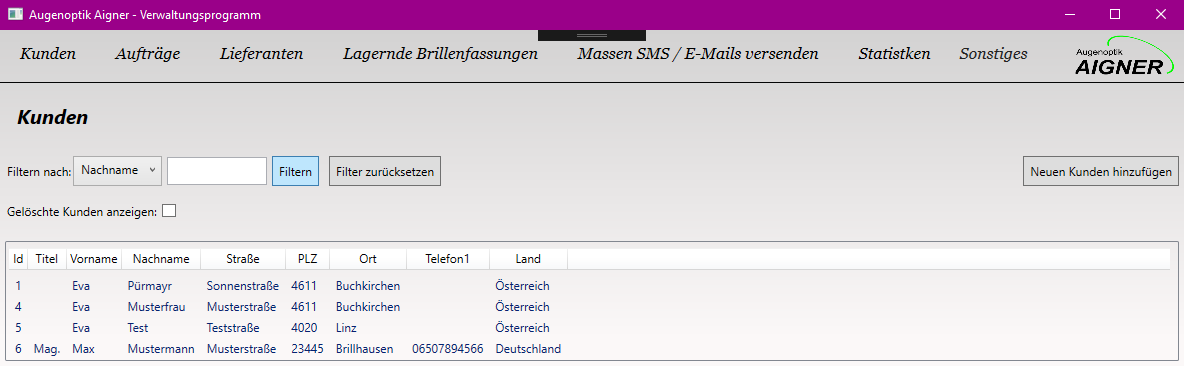
\includegraphics[scale=.45]{images/Kunden.png}
\end{center}
	\caption{Screenshot der Kundenverwaltung}
	\label{fig:sample}
\end{figure}
Beim Klick des Buttons ''Neuen Kunden hinzufügen'' erscheint ein neues Fenster, welches einen neuen Kunden erstellt. Hier kann der Benutzer weitere Daten eingeben, wie beispielsweise Hobbies, Job oder den Geburtstag. Außerdem kann der Benutzer den Ort und das Land aus einer Drop-Down-List auswählen. Falls der Ort bzw. das Land noch nicht vorhanden ist, kann der Benutzer auf den danebenliegenden Knopf drücken und einen neuen Ort/Land anlegen. 
\begin{figure}[H]
\begin{center}
	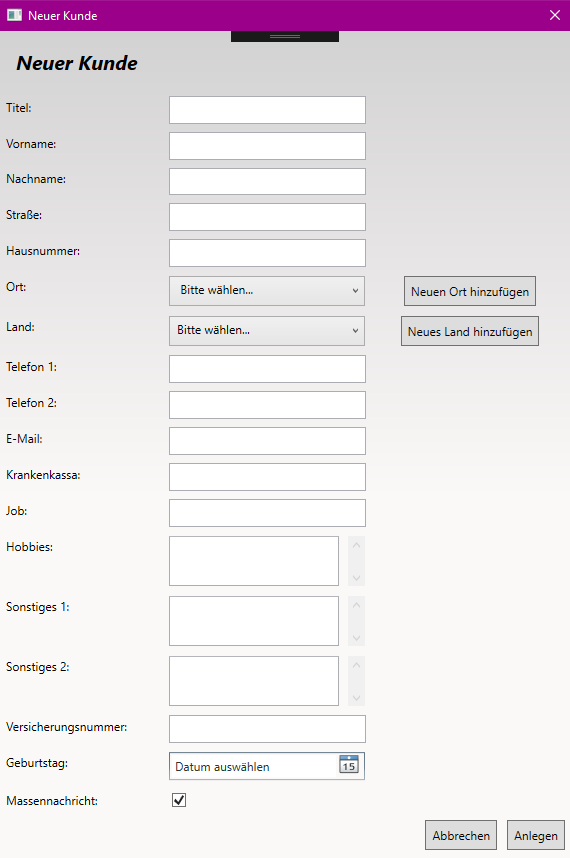
\includegraphics[scale=.4]{images/NeuerKunde.png}
\end{center}
	\caption{Screenshot Neuen Kunden anlegen}
	\label{fig:sample}
\end{figure}
Falls der Benutzer nach dem Anlegen des Kunden noch Änderungen vornehmen möchte, kann er dies auf der Startseite durch einen Doppelklick auf den gewünschten Kunden erledigen. Dadurch erscheint ein neues Fenster, auf welchem der Benutzer alle Daten des Kunden bearbeiten kann und zusätzlich alle Bestellungen des Kunden sieht. Außerdem besteht hier die Möglichkeit den Kunden zu löschen. Damit ist allerdings aus datenbanktechnischen Gründen gemeint, den Kunden nicht mehr bearbeitbar zu machen, der Benutzer kann keinen Kunden wirklich löschen. Der Grund dafür ist, dass jede Bestellung in der Datenbank auf einen Kunden verweisen muss und wenn ein Kunde bereits mehrere Bestellungen getätigt hat und der Benutzer danach den Kunden löschen möchte, würden alle seine Bestellungen mitgelöscht werden. 
\begin{figure}[H]
\begin{center}
	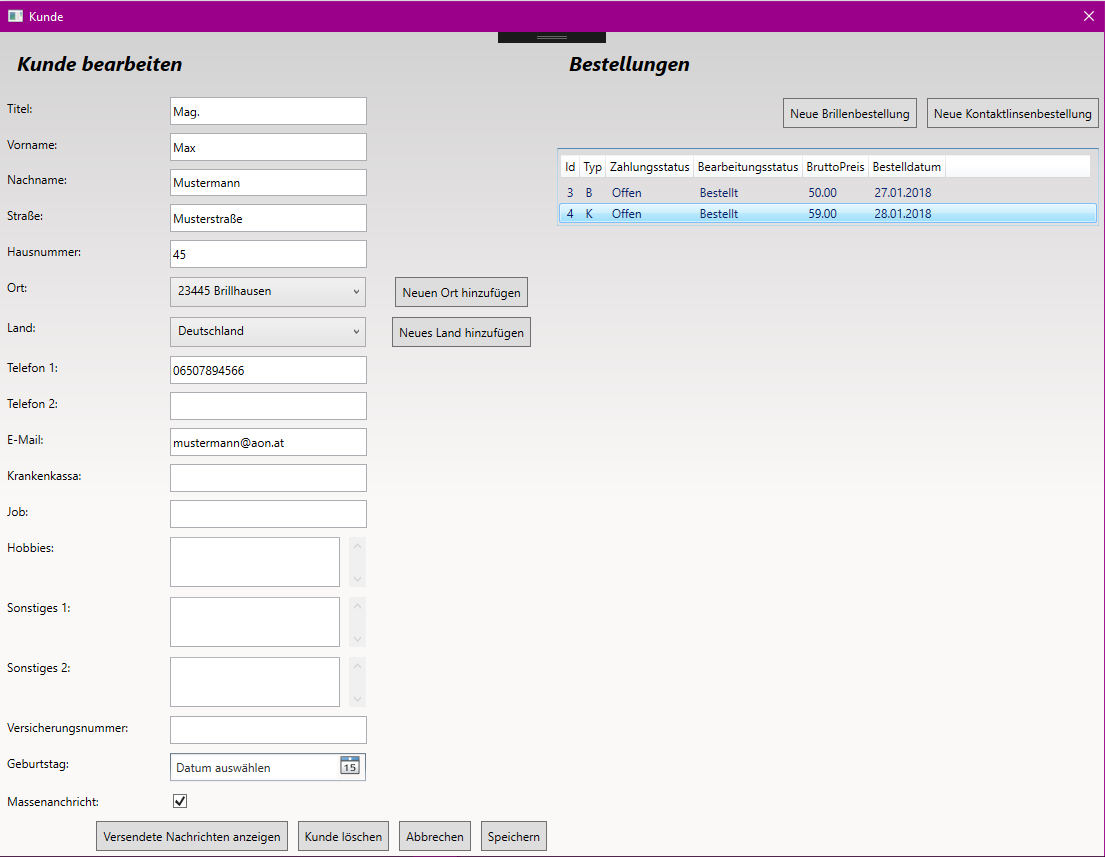
\includegraphics[scale=.25]{images/KundenDetails.png}
\end{center}
	\caption{Screenshot der Kundendetails}
	\label{fig:sample}
\end{figure}
Technischer Hintergrund:
Damit die Kunden auf der Startseite angezeigt werden können, müssen sie zuerst aus der Datenbank in eine ObservableCollection vom Typ Customer geladen werden. 
Danach wird auf Basis der Datensätze eine ICollectionView erstellt, welche die Daten dann anzeigt. Im Vergleich zur ObservableCollection bietet die ICollectionView beim Anzeigen viele Vorteile (siehe Kapitel 3.1.8). 
Um einen Kunden zu bearbeiten, muss das Objekt zuerst lokal kopiert werden.
\begin{lstlisting}
private Customer CopyCustomer(Customer item)
{
	Customer customer = new Customer();
	GenericRepository<Customer>.CopyProperties(customer, item);
	if (item.Town_Id != null)
	{
		Town town = new Town(); //Referenced town must be copied as well
		GenericRepository<Town>.CopyProperties(town, 	uow.TownRepository.GetById(item.Town_Id));
		customer.Town = town;
	}
	if (item.Country_Id != null)
	{
		Country country = new Country();
		GenericRepository<Country>.CopyProperties(country, uow.CountryRepository.GetById(item.Country_Id));
		customer.Country = country;
	}
	return customer;
}
\end{lstlisting}
Der Grund dafür ist, dass immer dieselbe Instanz von ''UnitOfWork'' verwendet wird. Wenn nur eine Referenz auf das Objekt erstellt werden würde, könnten die Änderungen nie rückgängig macht werden, weil sie ja immer sofort in die UnitOfWork-Instanz übertragen werden würden (siehe Kapitel 4.1.2).
\begin{lstlisting}
Customer cus = uow.CustomerRepository.GetById(1);
\end{lstlisting}
Damit ein Kunde gelöscht werden kann, enthält die Klasse Kunde eine Property namens 'Deleted', welche angibt, ob der Kunde gelöscht wurde. Wenn diese auf 'true' gesetzt wird, kann der Benutzer den Kunden durch die Checkbox auf der Startseite ausblenden. Falls er dies nicht tut, wird der Kunde auf der Startseite angezeigt, allerdings erscheint eine Fehlermeldung, wenn der Benutzer versucht die Detailseite des Kunden zu öffnen. Dadurch ist es auch unmöglich neue Bestellungen für diesen Kunden anzulegen oder die Daten des Kunden zu bearbeiten. Die Bestellungen des gelöschten Kunden werden trotzdem normal angezeigt.
\subsection{Auftragsverwaltung}
Grundsätzlich gibt es zwei Arten von Aufträgen: Brillen- und Kontaktlinsenaufträge. Eigentlich haben beide Arten dieselben Eigenschaften, nur der Brillenauftrag verweist auf eine Brillenfassung und der Kontaktlinsenauftrag nicht. Außerdem hat ein Brillenauftrag einen Brillentyp und ein Kontaktlinsenauftrag einen Kontaktlinsentyp. Damit kann der Benutzer beispielsweise unterscheiden, ob es sich um eine Fern- oder Nahbrille handelt. Generell wird streng zwischen Brillen- und Kontaktlinsenaufträgen unterschieden, deshalb werden unter dem Menüpunkt ''Aufträge'' auch zwei verschiedene Listen angezeigt. Jeder dieser Aufträge beinhaltet nur eine Brillen- oder Kontaktlinsenbestellung. Wie gewohnt kann man diese Listen wieder filtern und sortieren. Allerdings kann der Benutzer von dieser Sicht aus keine neuen Aufträge erfassen, dazu muss er in der Kundenverwaltung zuerst einen Kunden auswählen. 
\begin{figure}[H]
\begin{center}
	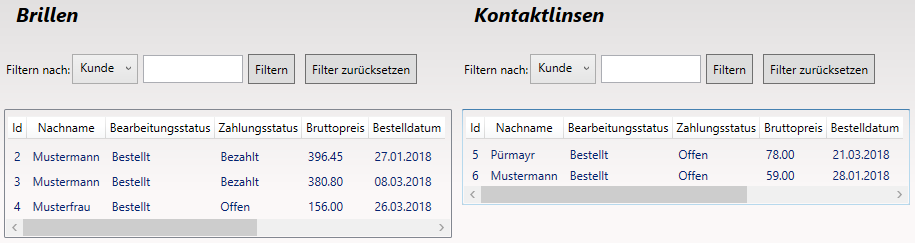
\includegraphics[scale=.45]{images/Auftraege.png}
\end{center}
	\caption{Screenshot der Auftragsverwaltung}
	\label{fig:sample}
\end{figure}
Wenn der Benutzer doppelt auf einen Auftrag klickt, erscheint entweder ein Detailfenster eines Brillenauftrags oder Kontaktlinsenauftrags. Im rechten Bereich des Fensters kann der Benutzer die einzelnen Preise der Komponenten angeben. Das Programm rechnet alle Preise  brutto und gibt zum Schluss die darin enthaltene Mehrwertsteuer an. Es wird nach folgender Formel gerechnet: Zuerst werden linker und rechter Glaspreis, Preis von Sonstigem und wenn vorhanden der Verkaufspreis der Brillenfassung addiert. Davon wird das Krankenkassageld abgezogen, der Selbstbehalt hinzugezählt und der Rabatt (dieser wird in Euro angegeben) wieder subtrahiert. Zwanzig Prozent davon sind schlussendlich die Mehrwertsteuer. 
Im unteren Bereich des Fensters kann der Benutzer Details zur Glasverarbeitung angeben. Wenn der Benutzer den Bearbeitungsstatus auf ''Abgeholt'' setzt, wird auch der Status der Brillenfassung in der Brillenfassungsverwaltung auf ''Verkauft'' gesetzt. \newline Der Benutzer hat die Möglichkeit zu jedem Auftrag einen Augenarzt zu vermerken. Von diesem Arzt wird allerdings nur der Name gespeichert. Der Benutzer kann nur aus einer Liste von Ärzten auswählen, welche er  selbst mittels dem Button 'Neuer Doktor' angelegt hat.
\begin{figure}[H]
\begin{center}
	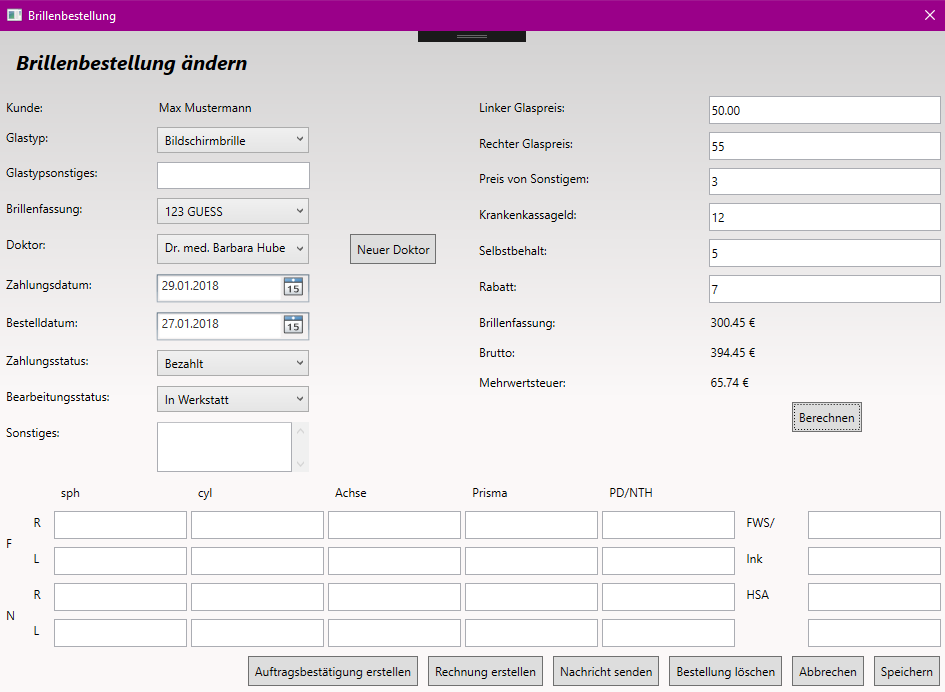
\includegraphics[scale=.3]{images/Brillenauftrag.png}
\end{center}
	\caption{Screenshot eines Brillenauftrags}
	\label{fig:sample}
\end{figure}
\subsubsection{Dokumente erstellen}
Unter den Angaben der Details zu den Gläsern, kann der Benutzer eine Auftragsbestätigung oder eine Rechnung erstellen. Die Dokumente werden als Word-Dokumente in einem Ordner abgespeichert. Das hat den Vorteil, dass der Benutzer selbst entscheiden kann, ob er noch etwas nachträglich ändern will oder das generierte Dokument gleich ausdruckt oder versendet. Gleichzeitig hat das Benutzen eines Word-Dokuments auch einen großen Nachteil, denn wenn der Benutzer nachträglich etwas ändert, wird diese Information nicht in das System weitergeleitet und somit könnten die erstellten Dokumente und der Auftrag selbst nicht dieselben Informationen beinhalten. Außerdem wird in der Datenbank immer nur der Pfad der zuletzt erstellten Rechnung/Auftragsbestätigung gespeichert. Das bedeutet, dass der Benutzer auch mehrere Dokumente zum selben Auftrag erstellen kann. Diese könnten sich auch voneinander unterscheiden, worüber das Programm ebenfalls keine Kontrolle hat. In diesem Fall wird nur ein Hinweis mit dem abgespeicherten Dokumentnamen angezeigt und gefragt ob das alte Dokument wirklich überschrieben werden soll.
\newline Damit das automatische Erstellen der Word-Dokumente funktioniert, muss der Benutzer  eine Word-Vorlage erstellen, die Felder enthält (MergeFields), welche das Programm ersetzen kann. Der Dokumentname der generierten Datei besteht immer aus der Bestell-Id, dem Dokumenttyp (Rechnung oder Auftragsbestätigung), dem Nachnamen des Kunden und dem aktuellen Datum. 
\newline Eine generierte Auftragsbestätigung könnte so aussehen:
\begin{figure}[H]
\begin{center}
	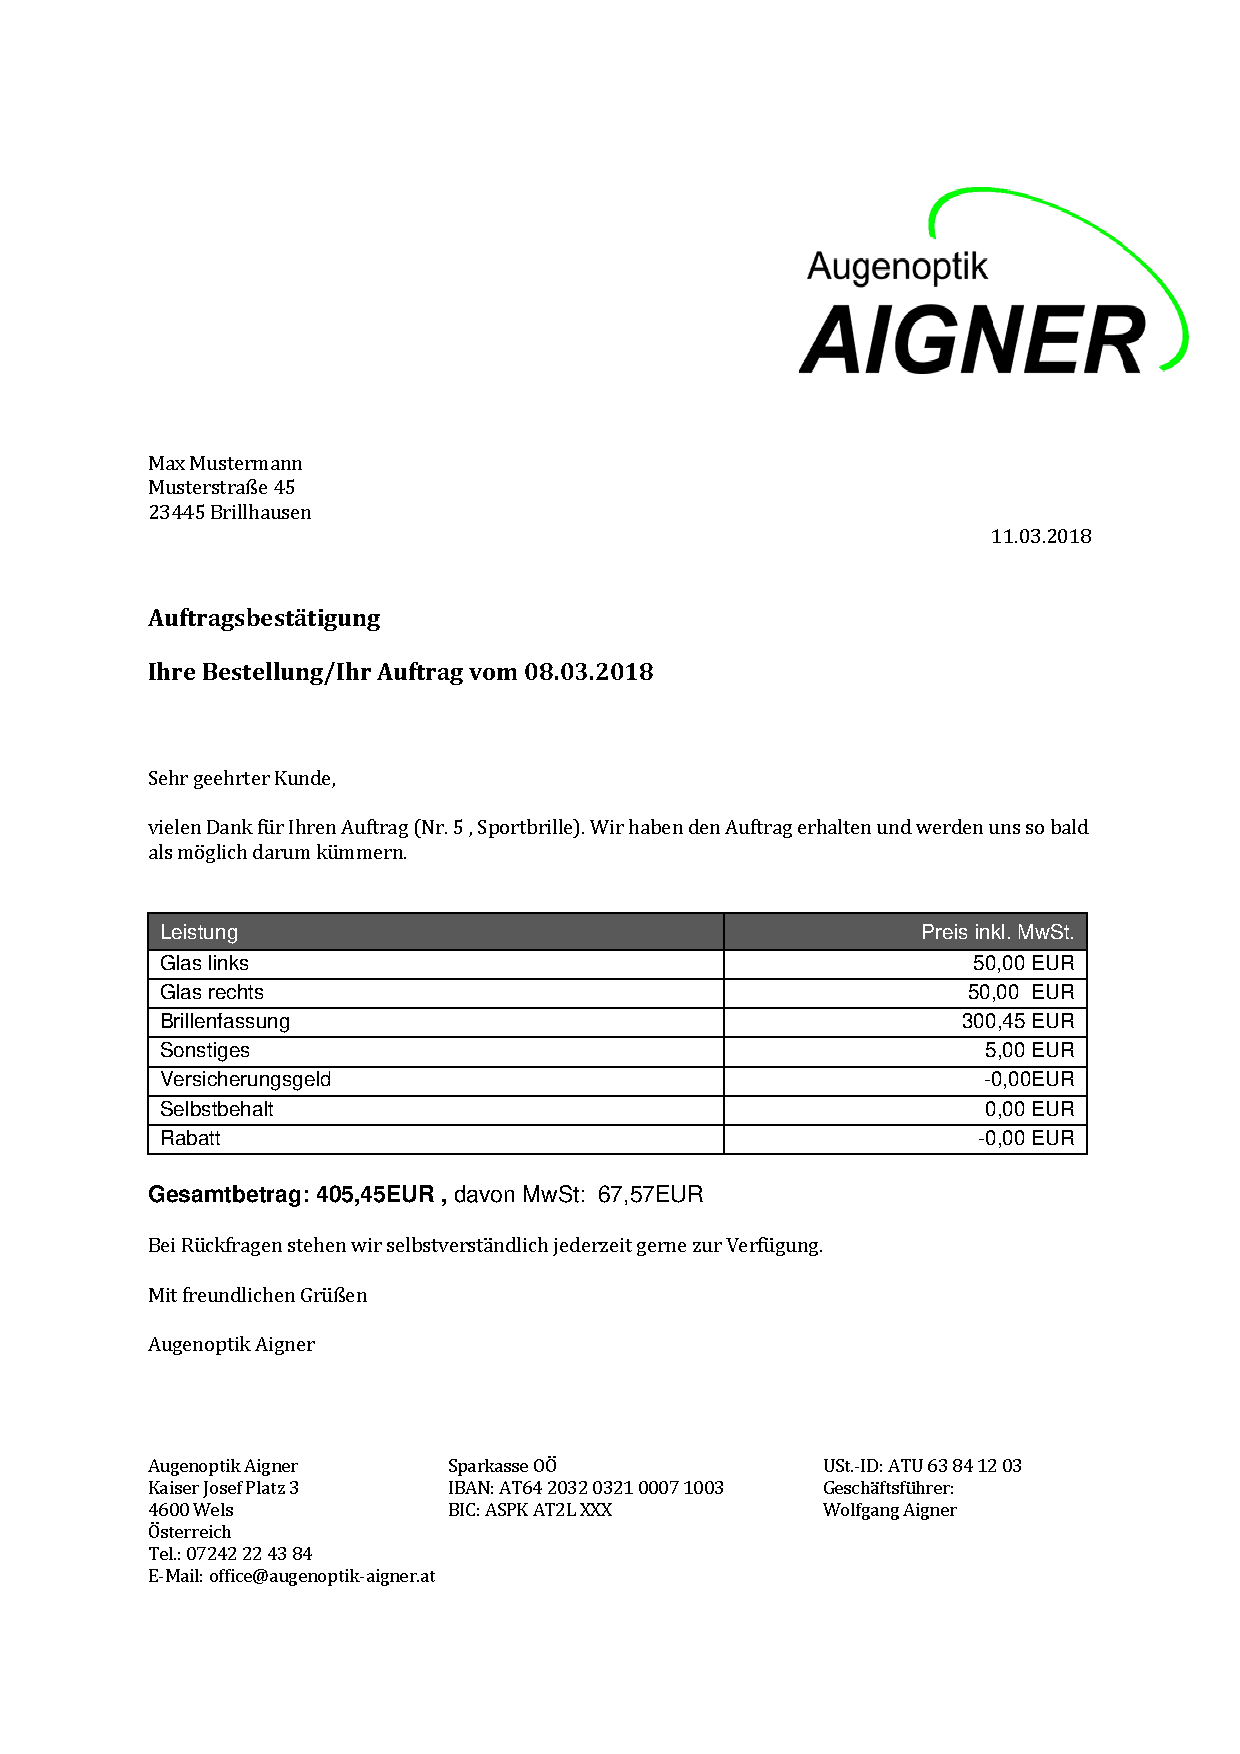
\includegraphics[scale=.75]{images/MusterAuftragsbestaetigung.pdf}
\end{center}
	\caption{Generierte Auftragsbest\"atigung}
	\label{fig:sample}
\end{figure}
Technischer Hintergrund:
Zur Erstellung von Word-Dokumenten wird Interop verwendet (siehe Kapitel 2.6). Die Methode CreateDocument benutzt eine vom Benutzer erstellte Wordvorlage und ersetzt die Mergefields. Der erste Parameter ''orderId'' gibt die Id der gewählten Bestellung an. Mit Hilfe dieser Nummer können aus der Datenbank die restlichen Daten geladen werden. Der Parameter oTemplatePath beschreibt den Pfad der Wordvorlage und der String path den Namen, unter dem das Dokument abgespeichert werden soll. Der Code unterhalb ist nur ein Ausschnitt der Methode.
\begin{lstlisting}
private static bool CreateDocument(int orderId, Object oTemplatePath, string path)
{
	Application wordApp = new Application();
	Document wordDoc = new Document();
	try
	{
		Order order;
		Customer cus;
		//Ausgeschnitten: Hier werden Order und Customer Werte aus der Datenbank zugewiesen 
		Object oMissing = System.Reflection.Missing.Value;
		wordDoc = wordApp.Documents.Add(ref oTemplatePath, ref oMissing, ref oMissing, ref oMissing);
		foreach (Field myMergeField in wordDoc.Fields)
		{
			Range rngFieldCode = myMergeField.Code;
		 	String fieldText = rngFieldCode.Text;
		 	
		 	//Nur Mergefields sollte bearbeitet werden
		 	if (fieldText.StartsWith(" MERGEFIELD")
		 	{
		 		string translatedFieldName;
		 		//Ausgeschnitten: Hier wird der Name der Property aus dem fieldText herausgeholt und auf Englisch uebersetzt
		 		string value = String.Empty;
		 		//Ausgeschnitten: Die Property wird in den Klassen gesucht und der Wert gespeichert z.B: Properties der Klasse Customer:
		 		if (typeof(Customer).GetProperty(translatedFieldName) != null)
		 		{
		 			value = cus.GetType().GetProperty(translatedFieldName).GetValue(cus, null)?.ToString();
		 		}
		 		myMergeField.Select();
		 		wordApp.Selection.TypeText(value);
		 	}
		 }
		 int idx = oTemplatePath.ToString().LastIndexOf("\\");
		 string p = oTemplatePath.ToString().Substring(0, idx + 1);
		 string completePath = p + path + ".docx";
		 wordDoc.SaveAs(completePath);
		 wordDoc.Close();
		 wordApp.Quit();
		 return true;
	}
	catch (Exception e)
	{
		Console.WriteLine(e);
		wordApp.Quit();
		wordDoc.Close();
		return false;
	}
}
\end{lstlisting}
Zuerst werden eine neue Applikation und ein neues Dokument erstellt. Nachdem der Auftrag und der Kunde aus der Datenbank geladen worden sind, wird die Vorlage für das Dokument geladen. Dabei ist nur der erste Parameter (''oTemplatePath'') von Bedeutung. Danach werden in einer Foreach-Schleife alle Felder des Dokumentes durchgegangen. Dabei werden nur jene bearbeitet, bei denen der Text des Feldes mit ''MERGEFIELD'' beginnt (es gibt auch Arten von Feldern in Word, jedoch sind in der Vorlage alle zu bearbeitenden Felder sogenannte Mergefields). Dann wird die gesuchte Property (Code ausgeschnitten) mit Hilfe der Variable ''fieldText'' ermittelt. ''fieldText'' muss aber zuerst auf Englisch übersetzt werden, da die Namen der Felder in der Vorlage deutsch sind, die Properties der Klassen aber Englisch. Der übersetzte Name der Property wird in der Variable ''translatedFieldName'' gespeichert. Anschließend werden allen Klassen nach dem Propertynamen durchsucht. Wenn die richtige Klasse gefunden wurde, wird der Wert der Property des Objekts in der Variable ''val'' gespeichert. Danach wird an Stelle des Mergefields in der Vorlage der ermittelten Wert eingetragen. Zum Schluss wird noch der gewünschte Pfad ermittelt und das Dokument unter diesem Pfad gespeichert.
Genau die selbe Methode wird benutzt, wenn eine Rechnung erstellt wird, die so aussehen könnte:
\begin{figure}[H]
\begin{center}
	\includegraphics[scale=.75]{images/Musterrechnung.pdf}
\end{center}
	\caption{Generierte Rechnung}
	\label{fig:sample}
\end{figure}
\subsection{Lieferantenverwaltung}
Ebenso wie für die Kunden, gibt es auch eine Verwaltung für die Lieferanten des Benutzers. Auch die Lieferanten lassen sich filtern und sortieren (siehe Kapitel Filtern und Sortieren). Lieferanten haben folgende Attribute: Name, Ort, Land, Adresse, FAX, Telefon, E-Mail, Kundennummer (damit ist die Id des Benutzers beim jeweiligen Lieferanten gemeint), Kontaktperson, Produkte und Sonstiges. Einen neuen Lieferant kann man mittels dem Button links oben anlegen und Lieferanten bearbeiten und löschen kann der Benutzer durch einen Doppelklick auf den gewünschten Lieferanten.
\begin{figure}[H]
\begin{center}
	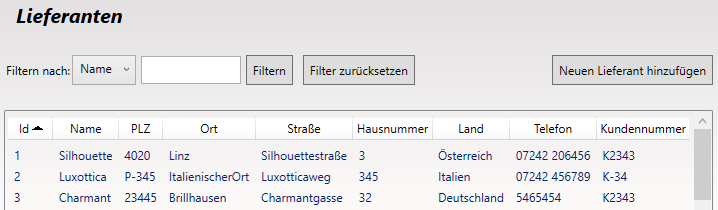
\includegraphics[scale=.45]{images/Lieferanten.png}
\end{center}
	\caption{Screenshot der Lieferantenverwaltung}
	\label{fig:sample}
\end{figure}
\subsection{Verwaltung der lagernden Brillenfassungen}
Genau wie bei der Verwaltung der Kunden und der Lieferanten gibt es auch eine Verwaltung der lagernden Brillenfassungen. Jede Brille die der Optiker verkauft, hat eine eigene Fassung und die wird hier erfasst. Dabei hat jede Brillenfassung folgende Attribute: Modell, Marke, Farbe, Größe, Status (bestellt, lagernd oder verkauft), Einkaufspreis, Einkaufsdatum, Verkaufspreis, Verkaufsdatum und der Lieferant. Die Liste kann wie gewohnt gefiltert und sortiert werden. Um eine neue Brillenfassung zu erfassen kann der Benutzer auf den Button links oben klicken und um eine bestehende Brillenfassung zu bearbeiten oder zu löschen muss der Benutzer einen Doppelklick auf die gewünschte Brillenfassung tätigen.
\newline Eigentlich würde man erwarten, dass zu den Brillenfassungen auch die Anzahl an lagernden Stück abgespeichert wird. Allerdings wurde dieses Feature nach Absprache mit dem Auftraggeber nicht implementiert, da jede Brillenfassung für jeden Auftrag einzeln bestellt wird. Deswegen wird auch der Status der Brillenfassung gespeichert.
\begin{figure}[H]
\begin{center}
	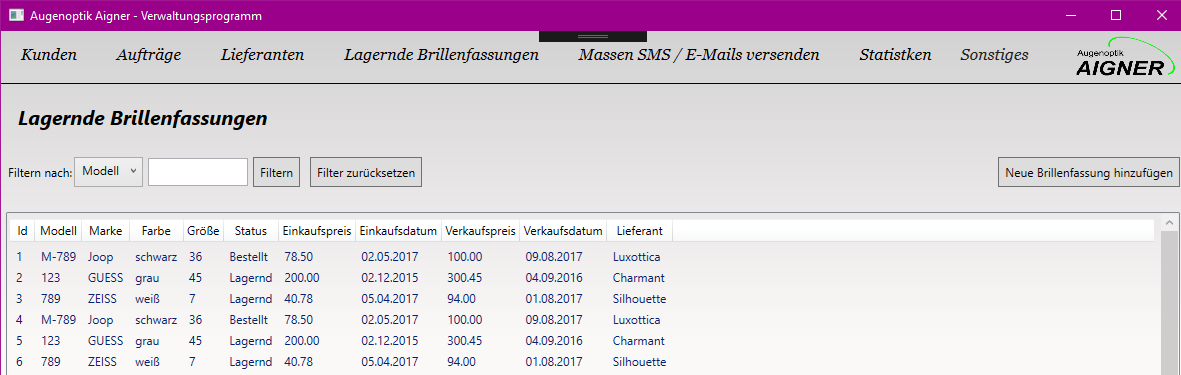
\includegraphics[scale=.45]{images/Brillenfassungen.png}
\end{center}
	\caption{Screenshot der lagernden Brillenfassungen}
	\label{fig:sample}
\end{figure}
\subsection{E-Mail und SMS}
\subsubsection{Massennachrichten}
Um regelmäßige Info- und Werbenachrichten auszusenden, bietet das Programm die Möglichkeit E-Mails oder SMS an alle Kunden zu versenden. Falls ein Kunde diese Nachrichten nicht mehr erhalten möchte, kann das der Benutzer bei dem einzelnen Kunden eintragen.
\subsubsection{E-Mail}
Wenn der Benutzer eine Massenmail versenden möchte, kann er einen Betreff und eine Nachricht eingeben, die nachher an alle Kunden gesendet wird. Als E-Mail-Adresse, wird die abgespeicherte Adresse des Kunden verwendet. Falls keine E-Mail-Adresse angegeben wurde, wird eine entsprechende Fehlermeldung angezeigt.

\begin{figure}[H]
\begin{center}
	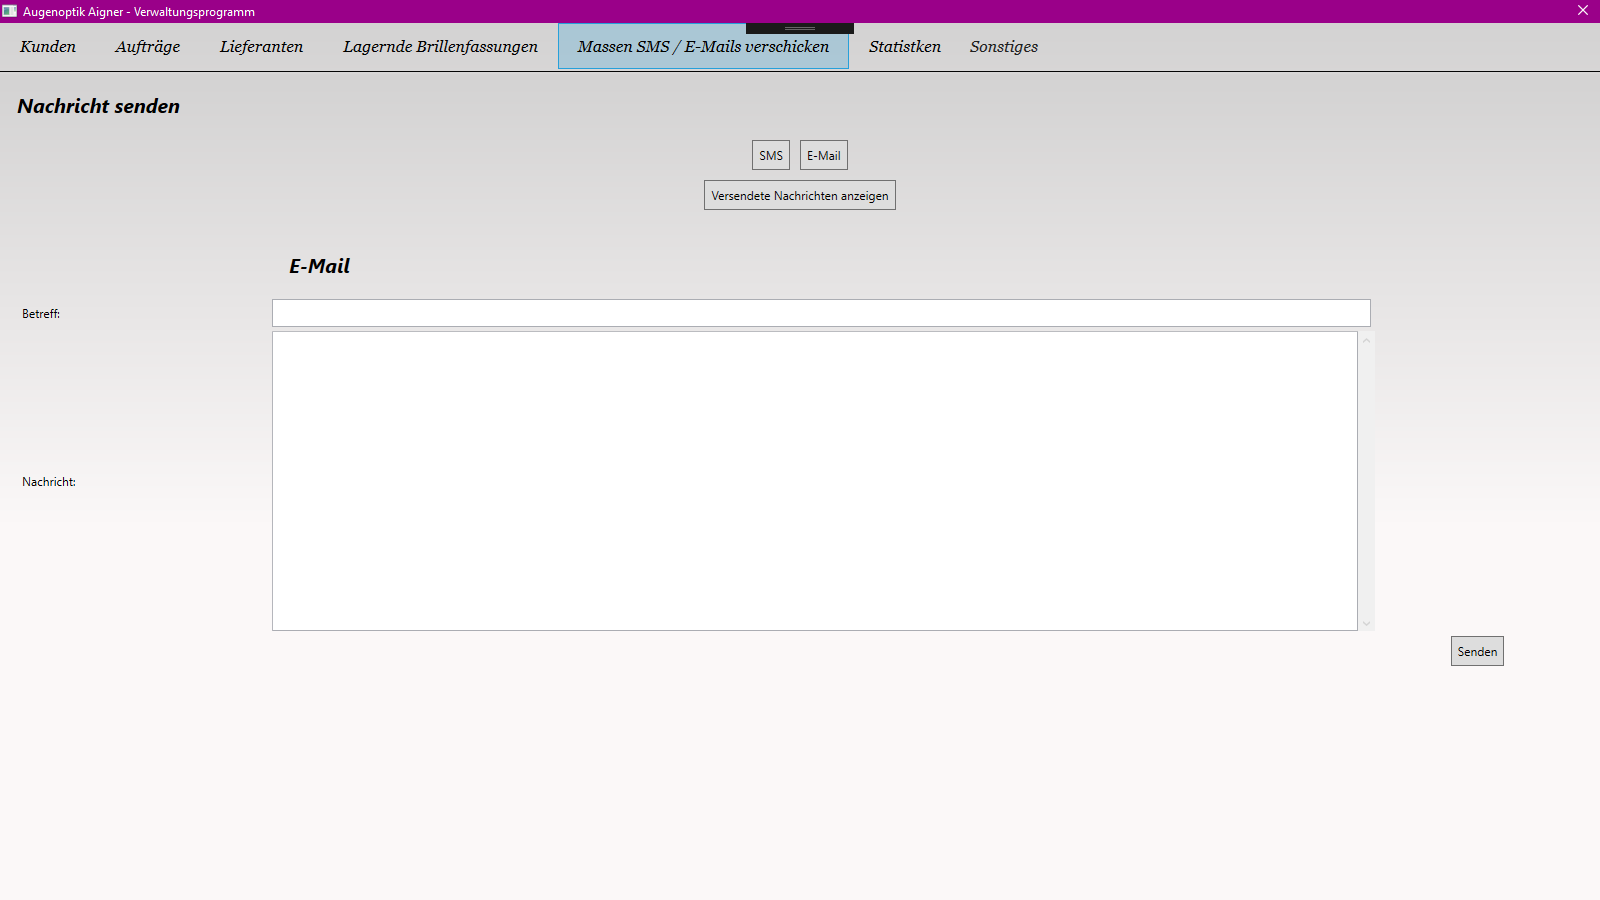
\includegraphics[scale=.4]{images/Massenemail.png}
\end{center}
	\caption{Screenshot der Massen E-Mails}
	\label{fig:sample}
\end{figure}
\underline{Technischer Hintergrund:}
\medskip
\linebreak
Es wird für jeden Kunden die gleiche Mail erstellt (Klasse MailMessage vom Namespace System.Net.Mail). Diesem Objekt werden Attribute wie Sender, Empfänger, Betreff, Nachricht usw. gesetzt und mittels eines SMTP-Clients versendet (Klasse SmtpClient ebenfalls vom Namespace System.Net.Mail). Der Smtp-Client bekommt noch Informationen wie Host, Port und natürlich die E-Mail-Adresse, von der die E-Mail weggeschickt werden soll, sowie das Passwort für die E-Mail-Adresse. In diesem Fall wurde eine Gmail-Adresse verwendet, die extra für diesen Zweck erstellt wurde.

\begin{lstlisting}
var message = new MailMessage();
message.To.Add(new MailAddress(item.Email));
message.From = new MailAddress("infodienst.augenoptikaigner@gmail.com");
message.Subject = this.Subject;
message.Body = this.Message;
this.Recipients.Add(new CustomRecipient() { Customer = item, Address = item.Email });

using (var smtp = new SmtpClient())
{
	var credential = new NetworkCredential
	{
		UserName = "infodienst.augenoptikaigner@gmail.com",
		Password = //not shown here
	};
	smtp.Credentials = credential;
	smtp.Host = "smtp.gmail.com";
	smtp.Port = 587;
	smtp.EnableSsl = true;
	await smtp.SendMailAsync(message);
}       
\end{lstlisting}
\bigskip
Danach wird die gesendete Nachricht noch in die Datenbank abgespeichert, damit der Benutzer später einen Überblick über alle gesendeten Nachrichten hat.

\subsubsection{SMS}
Zum Versenden der SMS wird der SMS-Dienst MessageBird verwendet (siehe Kapitel 2.8). Ähnlich wie beim Versenden einer E-Mail, gibt der Benutzer wieder eine Nachricht ein, allerdings kann er keine Betreff einfügen.
\begin{figure}[H]
\begin{center}
	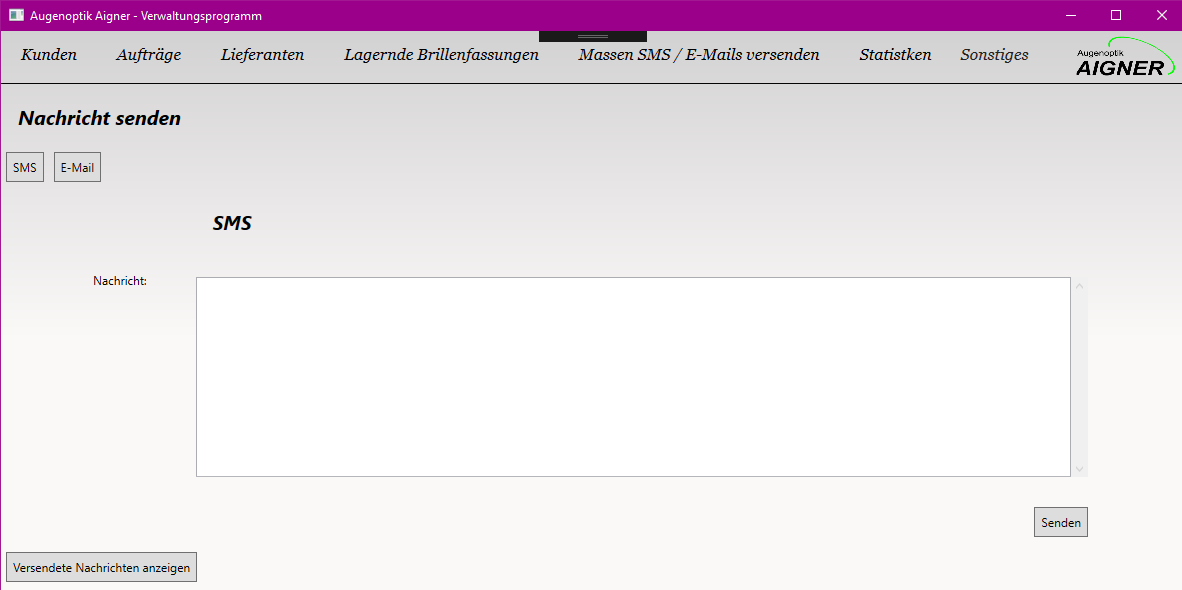
\includegraphics[scale=.4]{images/Massensms.png}
\end{center}
	\caption{Screenshot der Massen SMS}
	\label{fig:sample}
\end{figure}
Diese Nachricht wird dann an alle Kunden gesendet, außer jene, bei denen eingetragen ist, dass sie keine Massennachricht mehr erhalten wollen. Als Telefonnummer wird standardmäßig die Telefonnummer 1 gewählt, außer diese ist nicht vorhanden, dann wird die Telefonnummer 2 gewählt. Die ausgewählte Nummer sollte eine mobile Telefonnummer (kein Festnetz) sein, sonst kann die Nachricht nicht versendet werden.
\begin{comment}
\newpage
\underline{Technischer Hintergrund:}
\linebreak
\linebreak 
Zum Senden einer Nachricht werden folgende Schritte benötigt:
\begin{lstlisting}
IProxyConfigurationInjector proxyConfigurationInjector = null;
Client client = Client.CreateDefault(AccessKey, proxyConfigurationInjector);
\end{lstlisting}
Und zum Versenden einer Nachricht:
\begin{lstlisting}
MessageBird.Objects.Message message = client.SendMessage(Properties.Settings.Default.SmsSenderText, this.Message, numbers);
\end{lstlisting}
Der AccessKey ist ein normaler String, der von MessageBird erstellt wird. Dabei kann jeder Benutzer von MessageBird mehrere AccessKeys bekommen, beispielsweise einen für Test-Nachrichten, die dann nicht versendet werden oder einen Key, mit dem dann echte SMS versendet werden. Der erste Parameter der Methode ''SendMessage'' beschreibt der Name der angezeigt werden soll, wenn ein Kunde die Nachricht empfängt. Dieser kann vom Benutzer geändert werden (siehe Kapitel 3.1.7).
Für jede Nachricht die versendet wird, wird das Guthaben auf MessageBird dementsprechend verringert. Sollte das Guthaben auslaufen, wird eine Fehlermeldung angezeigt.
\end{comment}

\subsubsection{Einzelne Nachrichten}
Dieselben Vorgänge werden auch verwendet um einzelne Nachrichten zu versenden. Dazu muss der Benutzer auf die Detailseite einer Bestellung klicken und dann auf „Nachricht senden“. Standardmäßig wird ein Text eingefügt, der dem Kunden mitteilt, dass seine Bestellung nun abholbereit ist. Der Standardtext kann vom Benutzer allerdings geändert werden (siehe Kapitel 3.1.7). Falls der Benutzer jedoch einmal einen ganz anderen Text versenden wollen, kann der Benutzer die Nachricht natürlich auch verändern.
\begin{figure}[H]
\begin{center}
	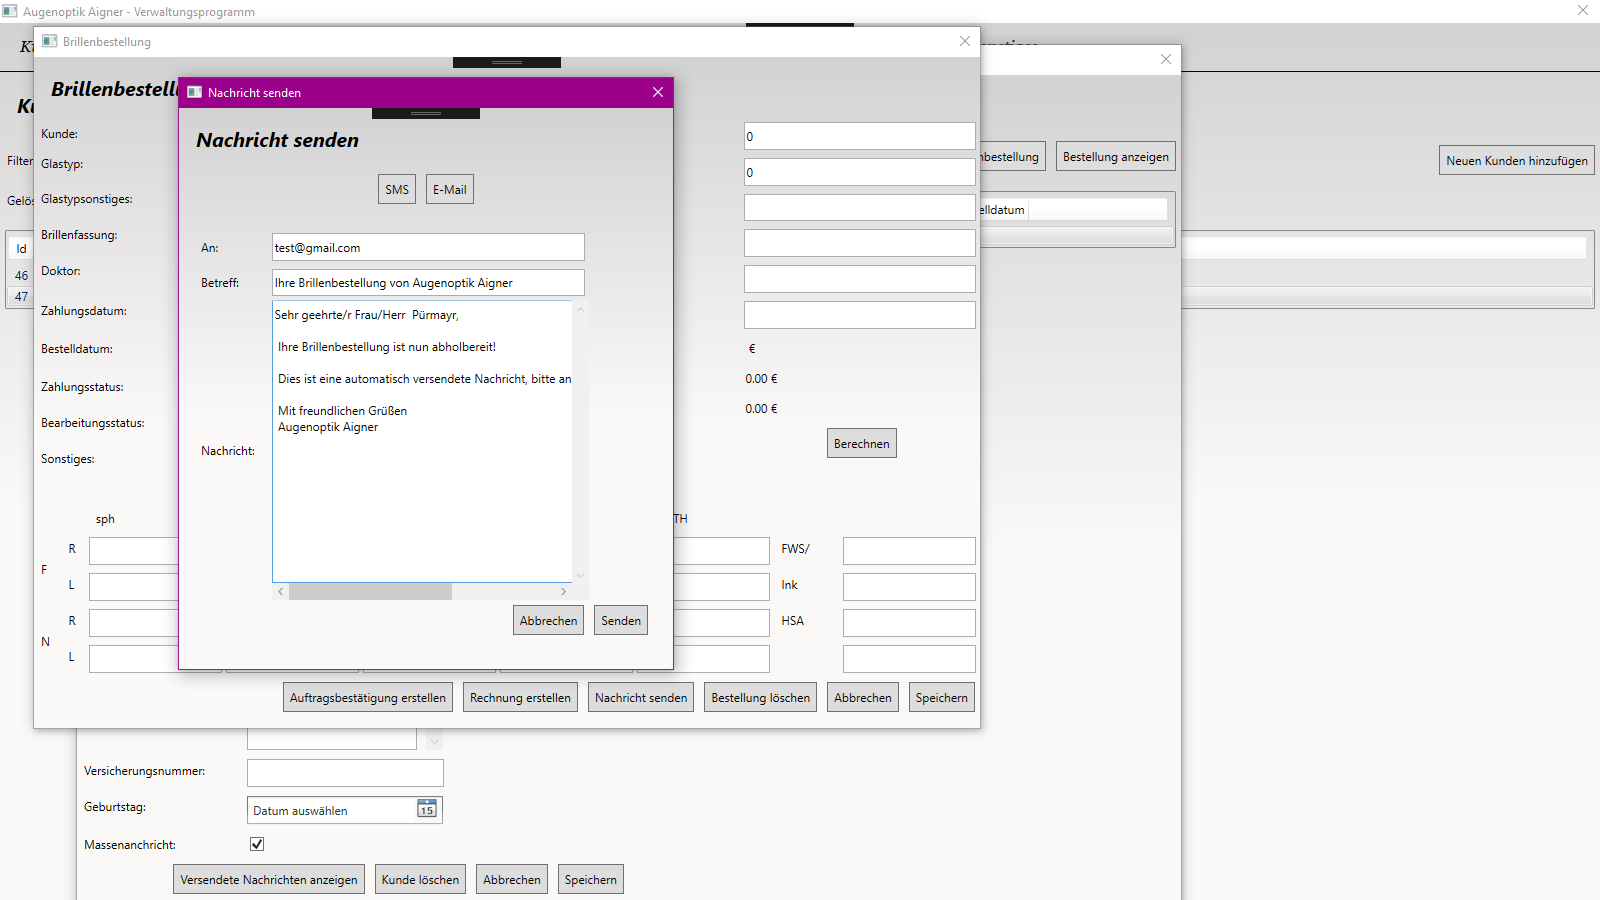
\includegraphics[scale=.4]{images/EinzelneNachricht.png}
\end{center}
	\caption{Screenshot der einzelnen Nachricht}
	\label{fig:sample}
\end{figure}
\subsubsection{Versendete Nachrichten}
Außerdem ist es möglich, alle Nachrichten, die vom System aus gesendet worden sind, anzuzeigen. Um nur Nachrichten anzuzeigen, die an einen bestimmten Kunden gesendet worden sind, muss der Benutzer auf die Detailseite eines Kunden klicken und dann die „Versendeten Nachrichten“ anzeigen. Falls der Benutzer alle Nachrichten sehen will, die er versendet hat, kann er diese unter dem Menüpunkt „Massen SMS /E-Mails verschicken“ sehen.\\
Dazu wurden in der Datenbank extra die Tabellen ''CustomMessage'' und ''CustomRecipient'' angelegt, um alle Nachrichten und deren Empfänger abspeichern zu können. Hier wird beispielsweise eine Massensms gespeichert:
\begin{lstlisting}
var m = new CustomMessage();
m.Date = DateTime.Now;
m.MessageText = this.Message;
m.MessageType = OpticiatnMgr.Core.Entities.MessageType.SMS;
m.Recipients = new List<CustomRecipient>();
var numbers = GetPhoneNumbers();
for (int i = 0; i < this.Customers.Count; i++)
{
	m.Recipients.Add(new CustomRecipient() { Customer = this.Customers[i], Address = numbers[i].ToString() });
}
uow.MessageRepository.Insert(m);
uow.Save();
\end{lstlisting}
\begin{figure}[H]
\begin{center}
	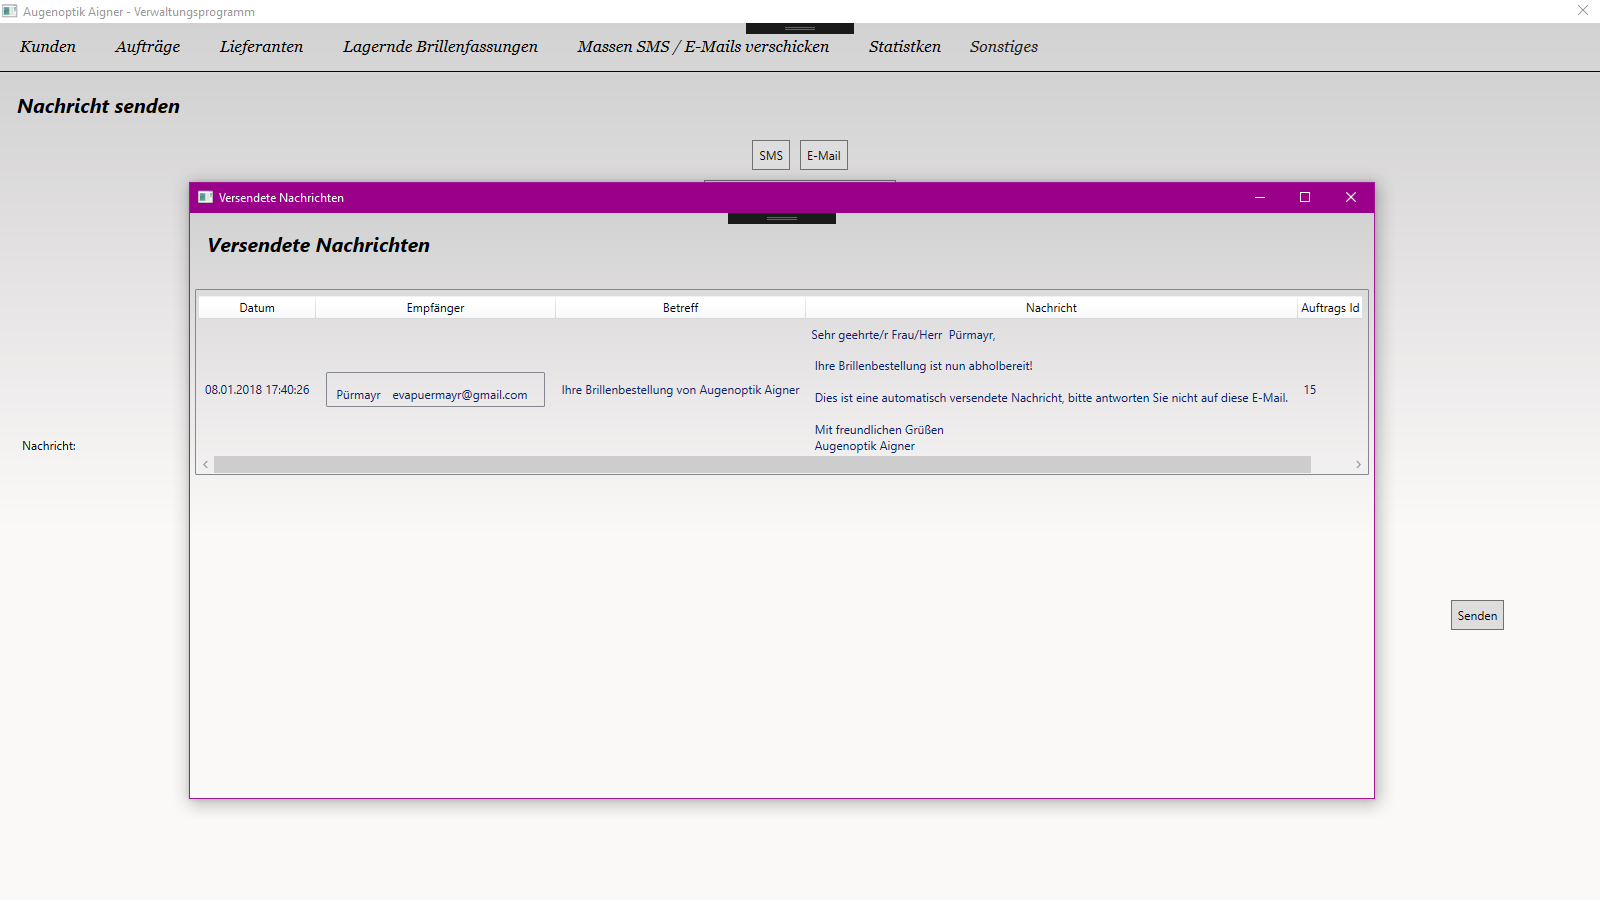
\includegraphics[scale=.5]{images/VersendeteNachrichten.png}
\end{center}
	\caption{Screenshot der versendeten Nachrichten}
	\label{fig:sample}
\end{figure}

\subsection{Statistiken}
Unter dem Menüpunkt ''Statistiken'' erhält der Benutzer eine Übersicht über alle verkauften Brillen und Kontaktlinsen. Dazu wird ein Liniendiagramm der verkauften Brillen/Kontaktlinsen von diesem Jahr und dem Jahr davor angezeigt. Damit ein Brillen/Kontaktlinsenauftrag in der Statistik mitberücksichtigt wird, muss ein Zahlungsdatum angegeben werden und der Bezahlungsstatus muss auf „Bezahlt“ gesetzt werden.
\begin{figure}[H]
\begin{center}
	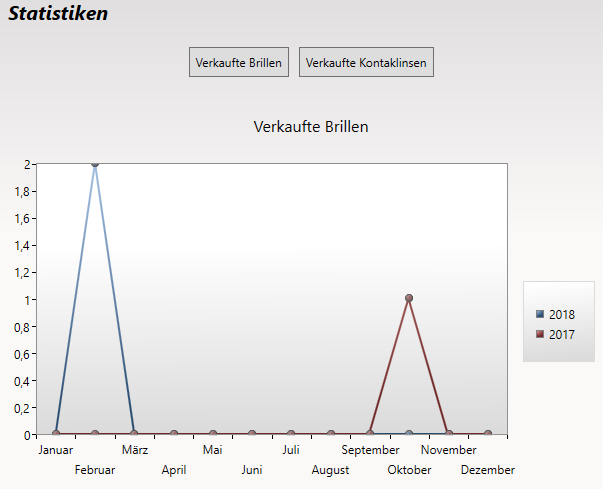
\includegraphics[scale=.4]{images/Statistiken.png}
\end{center}
	\caption{Screenshot der Statistiken}
	\label{fig:sample}
\end{figure}
\subsubsection{Technischer Hintergrund}
Zur Darstellung wurde das Wpf-Toolkit verwendet (siehe Kapitel 2.7).
\begin{comment} 
Dazu wird in dem .xaml File der Namespace angegeben: 
\begin{lstlisting}
<Page xmlns:toolkitCharting="clr-namespace:System.Windows.Controls
DataVisualization.Charting;assembly=System.Windows.Controls.DataVisualization
.Toolkit">
\end{lstlisting}
\end{comment}
Um ein Liniendiagramm zu erzeugen:
\begin{lstlisting}
<toolkitCharting:Chart Title="{Binding Title}">
            <toolkitCharting:LineSeries Title="{Binding NewYear}"  DependentValueBinding="{Binding Value}" IndependentValueBinding="{Binding Key}" ItemsSource="{Binding NewValues}"/>
            <toolkitCharting:LineSeries Title="{Binding OldYear}"  DependentValueBinding="{Binding Value}" IndependentValueBinding="{Binding Key}" ItemsSource="{Binding OldValues}"/>
</toolkitCharting:Chart>
\end{lstlisting}
Dabei sind ''NewValues'' und ''OldValues'' vom Typ: 
\begin{lstlisting}
public ObservableCollection<KeyValuePair<string, int>> NewValues { get; set; }
public ObservableCollection<KeyValuePair<string, int>> OldValues { get; set; }
\end{lstlisting}
Die Daten werden mittels Linq (Kapitel 2.1.1) erfasst.
\subsection{Sonstiges}
Unter dem Menüpunkt ''Sonstiges'' erscheinen vier Unterpunkte: 
\begin{itemize}
\item Orte bearbeiten
\item Länder bearbeiten
\item Brillentypen bearbeiten
\item Kontaktlinsentypen bearbeiten
\item Vorgegebene Texte bearbeiten
\end{itemize}
Wie die Überschriften schon vermuten lassen, öffnen die vier oberen Buttons jeweils ein eigenes Fenster, welches eine Übersicht über alle vorhandenen Objekte zeigt. Am Beispiel ''Länder'' wird nun die Verwendung gezeigt:
\begin{figure}[H]
\begin{center}
	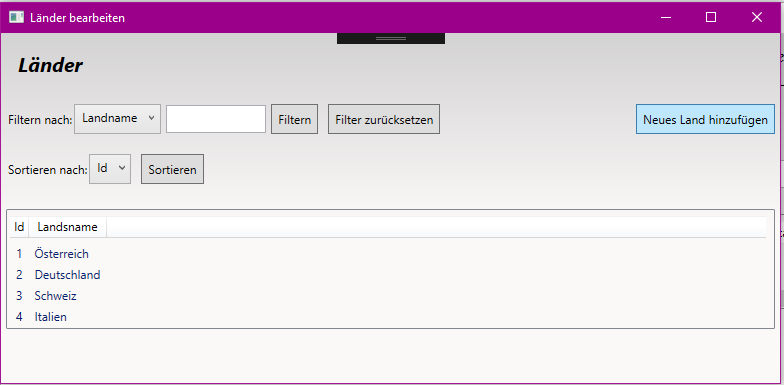
\includegraphics[scale=0.75]{images/Laender.png}
\end{center}
	\caption{Screenshot der L\"ander}
	\label{fig:sample}
\end{figure} 
Im oberen Bereich können die Länder nach Name oder Id gefiltert werden. Allerdings funktioniert das Sortieren hier anders als bei den Übersichtlisten. Der Benutzer kann auswählen, nach was er gerne sortieren möchte und danach sortiert das Programm aufsteigend nur nach dieser einen Property. Mit einem Doppelklick kann ein Land bearbeitet/gelöscht werden und rechts oben kann ein neues Land hinzugefügt werden.
\begin{figure}[H]
\begin{center}
	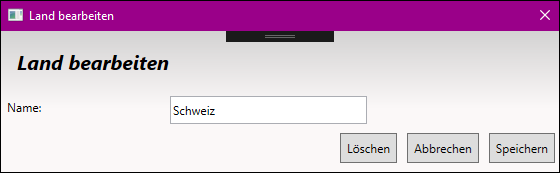
\includegraphics[scale=0.75]{images/LandBearbeiten.png}
\end{center}
	\caption{Land bearbeiten}
	\label{fig:sample}
\end{figure} 
\subsubsection{Vorgegebene Texte bearbeiten}
Unter diesem Menüpunkt können Texte, die standardmäßig im Programm vorgeschlagen werden, bearbeitet werden. Dazu gehören sämtliche Texte und bei E-Mails auch Betreffe, die beim Versenden einer einzelnen Nachricht vorgeschlagen werden. Außerdem kann auch der Name bearbeitet werden, der Kunden angezeigt wird, wenn sie eine SMS vom Programm aus erhalten. Bei allen Texten außer dem Sendernamen von SMS, hat der Benutzer die Möglichkeit die Nachrichten zu personalisieren. Dazu muss er nur an der Stelle, an dem zum Beispiel der Nachname des Kunden eingefügt werden soll ''\{3\}'' schreiben. Außerdem kann der Benutzer auch Zeilenumbrüche einfügen, damit beispielsweise in einer E-Mail nicht nur eine einzige Zeile Text steht.
\begin{figure}[H]
\begin{center}
	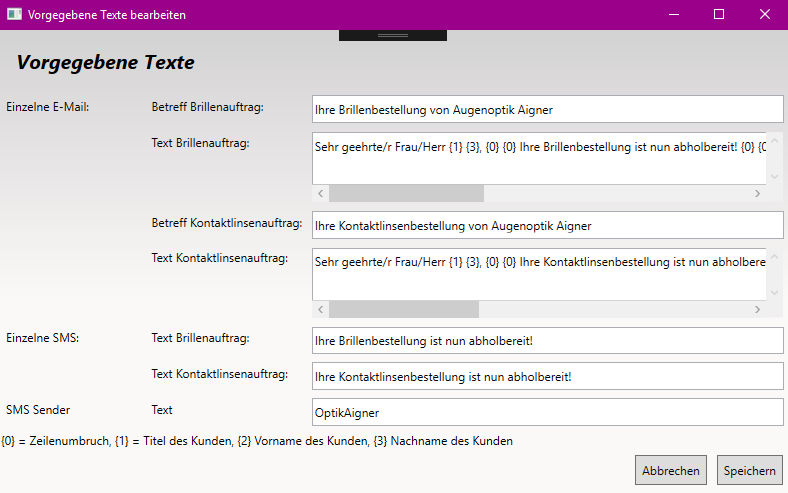
\includegraphics[scale=0.75]{images/VorgegebeneTexteBearbeiten.png}
\end{center}
	\caption{Vorgegebene Texte bearbeiten}
	\label{fig:sample}
\end{figure} 
\underline{Technischer Hintergrund}: Um diese Informationen zu speichern, werden sogenannte User-Settings verwendet. Diese sind in den Properties des Projektes unter dem Punkt ''Settings'' eingetragen und haben die Eigenschaft, dass sie nicht zurückgesetzt werden, sobald das Programm beendet wird. In diesen ''Settings'' kann der Name der Einstellung, der Typ (in dieser Arbeit wird nur der Typ string benötigt), der Geltungsbereich und der Wert  eingetragen werden. Der Geltungsbereich kann entweder ''Application'' oder ''User'' sein. Der Unterschied besteht darin, dass ''Application''-Einstellungen zur Laufzeit nicht verändert werden können und ''User''-Einstellungen schon. Deshalb sind alle Einstellungen dieser Arbeit ''User''-Einstellungen.
\newline Im Code des ViewModels sind Properties zu den zu bearbeitenden Texten vorhanden, welche im Getter nur die passende Einstellung zurückliefern und im Setter diesen Text speichern. Die nachfolgende Property beschreibt den Text im Betreff, der angezeigt wird, wenn eine einzelne E-Mail an einen Kunden mit einem Brillenauftrag versendet wird.
\begin{lstlisting}
public string SingleEmailSubjectGlassesOrder 
{
	get 
	{ 
		return Properties.Settings.Default.SingleEmailSubjectGlassesOrder; 
	} 
	set 
	{ 
		Properties.Settings.Default.SingleEmailSubjectGlassesOrder = value; 
	} 
}
\end{lstlisting}
Bevor das Fenster mit ''Speichern'' geschlossen wird, muss unbedingt folgende Methode aufgerufen werden. Ansonsten werden die Änderungen nicht gespeichert und beim nächsten Programmstart werden wieder die alten Texte angezeigt.
\begin{lstlisting}
Properties.Settings.Default.Save();
\end{lstlisting}
Falls der Benutzer die Änderungen nicht speichern möchte kann er den ''Abbrechen''-Button betätigen. Dann muss allerdings nachfolgende Methode aufgerufen werden, ansonsten bleiben die Änderungen bis zum Schließen des Programms erhalten. Erst beim nächsten Programmstart werden sie wieder zurückgesetzt.
\begin{lstlisting}
Properties.Settings.Default.Reload();
\end{lstlisting}
\subsection{Filtern und Sortieren}
\subsubsection{Filtern}
Auf allen Hauptseiten der Applikation (Kunden, Brillen- und Kontaktlinsenaufträge, Lieferanten, Lagernde Brillenfassungen) sowie auf den Seiten unter dem Menüpunkt „Sonstiges“ (Orte, Länder, Brillen- und Kontaktlinsentypen) ist es möglich die Datensätze zu filtern. Dies passiert immer nach demselben Schema, dennoch ist diese Funktion für jede dieser Seiten einzeln implementiert.
Dazu muss der Benutzer das Feld aussuchen, nach welchem er gerne filtern möchte, danach einen Text eingeben und dann auf „Filtern“  oder die Taste „Enter“ drücken. Das Programm gibt nun nur jene Datensätze aus, bei denen das gewünschte Feld den eingegebenen Text enthält. Neben dem „Filtern“-Button befindet sich ein „Filter löschen“-Button, der wieder alle Datensätze zum Vorschein bringt.
\begin{figure}[H]
\begin{center}
	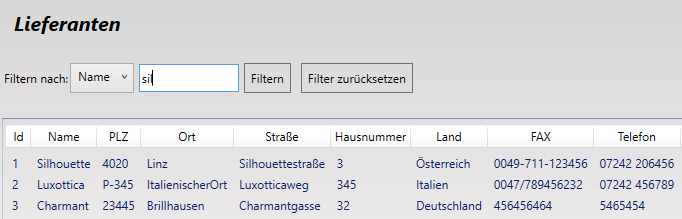
\includegraphics[scale=0.75]{images/filter.png}
\end{center}
	\caption{Screenshot des Filters}
	\label{fig:sample}
\end{figure}
Im nachfolgenden Beispiel wird anhand der „Lagernden Brillenfassungen“ erklärt wie der Filter funktioniert. 
Im ViewModel gibt es ein Feld, welches ''PropertiesList'' heißt (vom Typ ObservableCollection\textless string\textgreater). In diesem werden alle Felder der jeweiligen Klasse aufgezählt. Davor werden noch Felder, nach denen der Benutzer später nicht filtern sollte, herausgestrichen. Bei Referenzen auf andere Objekte, zum Beispiel bei der Brillenfassung der Lieferant, wird die ''Supplier\_Id'' entfernt, der String ''Supplier'' bleibt allerdings in der Liste. Später beim Übersetzen in Englisch wird überprüft, ob nach einem Fremdschlüssel gefiltert wird. In diesem Fall wird der Name des Fremdschlüssels (hier ''Supplier'') zu dem Hauptnamen in der Property umgewandelt (''SupplierName''). Das bedeutet, dass wenn der Lieferant als Filterfeld ausgewählt wird, in Wirklichkeit nur nach einem Feld (hier dem Namen des Lieferanten) gefiltert wird.
\newline Nachdem aller Felder ausgewählt wurden, wird jedes Feld in Deutsch übersetzt. Dies geschieht mittels einem kleinen Wörterbuch (Klasse ResourceManager), welches eine Übersetzung für jedes Feld bereithält. Die Wörter, die im ResourceManager stehen, müssen selbst eingefügt werden und werden in einem File namens ''Resources.resx'' unter den Properties des Projektes abgespeichert. Neben einfachen Wörtern könnten hier auch Bilder, Dateien oder Ähnliches verwaltet werden. Hier wird die Liste der Felder aus denen der Benutzer später sein „Filterfeld“ auswählen kann erstellt. 
\begin{lstlisting}
public ObservableCollection<String> PropertiesList { get; }

private ResourceManager manager = Properties.Resources.ResourceManager;

private ObservableCollection<string> GetAllProperties()
{
	ObservableCollection<string> props = new 							ObservableCollection<string>(typeof(EyeGlassFrame).GetProperties()
.Select(p => p.Name).ToList());
	ObservableCollection<string> newList = new ObservableCollection<string>();
	props.Remove("Timestamp"); //Shouldnt be able to filter by timestamp
   props.Remove("Supplier_Id"); //Shouldnt be able to filter by supplier_id
   foreach (var item in props)
   {
   		var germanItem = manager.GetString(item);
   		if (germanItem != null)
             newList.Add(germanItem);
   }
   return newList;
}
\end{lstlisting}
Wenn der Benutzer einen Text eingibt und danach „Filtern“ drückt, wird das Feld, das er gewählt hat zuerst mit Hilfe des ResourceManagers auf Englisch übersetzt.  Danach wird die Methode Filter() aufgerufen, die den passenden Filter setzt, falls der Benutzer einen Text eingegeben hat.
\begin{lstlisting}
public void Filter()
{
	try
	{
		if (!String.IsNullOrEmpty(this.FilterText))
		{
			this.EyeGlassFramesView.Filter = new Predicate<object>(Contains);
		}
		else
			this.EyeGlassFramesView.Filter = null;
	}
	catch (Exception e)
	{
		Console.WriteLine(e.StackTrace);
	}
}
\end{lstlisting}
Dabei muss man wissen, dass EyeGlassFramesView vom Typ ICollectionView ist. Diese Property wird im Konstruktor aus der Liste der wirklichen Brillenfassungen erzeugt (EyeGlassFrames). Der Typ ICollectionView ist als Anzeigeelement für Listen gedacht, weshalb es auch ein Feld namens „Filter“ gibt (Mehr dazu: \cite{microsoft_collectionview.filter-eigenschaft_2017}). Durch die Methode „Contains“ wird dieser auch gesetzt. Der folgende Code stammt aus dem ViewModel der lagernden Brillenfassung.
Properties:
\begin{lstlisting}
public ObservableCollection<EyeGlassFrame> EyeGlassFrames { get; set; }
public ICollectionView EyeGlassFramesView { get; set; }
public string TranslatedFilterProperty { get; set; }
public string FilterText { get; set; }
\end{lstlisting}
Im Konstruktor wird EyeGlassFramesView initialisiert.
\begin{lstlisting}
this.EyeGlassFramesView = CollectionViewSource.GetDefaultView(EyeGlassFrames);
\end{lstlisting}
Die Methode Contains gibt zurück, ob das Objekt „f“ dem angegebenen Filter entspricht. Dazu wird zunächst überprüft, ob die Klasse EyeGlassFrame die Property enthält, nach der der Benutzer filtert. Wenn ja, gibt die Methode zurück, ob in dieser Property die Zeichenkette vorkommt, nach der der Benutzer sucht. Danach überprüft das Programm ob die gesuchte Eigenschaft eine Eigenschaft der Klasse Supplier ist. Das passiert, weil jede lagernde Brillenfassung einen Lieferanten hat. Deswegen kann es sein, dass der Benutzer nach einer Eigenschaft filtert, die gar nicht in der Klasse EyeGlassFrame enthalten ist, sondern nur in der Klasse Supplier. Wenn keiner dieser Fälle zutrifft, was nicht vorkommen sollte, wird eine Fehlermeldung zurückgegeben.
\begin{lstlisting}
private bool Contains(object f)
{
	EyeGlassFrame frame = f as EyeGlassFrame;
	if (typeof(EyeGlassFrame).GetProperty(TranslatedFilterProperty) != null)
	{
		return frame.GetType().GetProperty(this.TranslatedFilterProperty)
		.GetValue(frame, null)?.ToString().ToUpper().IndexOf(this.FilterText.ToUpper()) >= 0;
	}
	else if (typeof(Supplier).GetProperty(TranslatedFilterProperty) != null) //Does the user filter by suppliername?
	{
		return frame.Supplier?.GetType()
		.GetProperty(this.TranslatedFilterProperty)
		.GetValue(frame.Supplier, null)?.ToString().ToUpper().IndexOf(this.FilterText.ToUpper()) >= 0;
	}
	else
	{
		MessageBox.Show("Beim Filtern ist ein Fehler aufgetreten!");
		return false;
	}
}
\end{lstlisting}
\subsubsection{Sortieren}
Bei den allen Hauptseiten, auf denen Daten angezeigt werden, ist eine dynamische Sortierung implementiert. Diese macht es dem Benutzer möglich, nach drei Spalten gleichzeitig auf- oder absteigend zu sortieren.  Dazu muss der Benutzer auf eine beliebige Spaltenüberschrift klicken. Das ist dann die Spalte, nach der zuerst aufsteigend sortiert wird. Drückt der Benutzer erneut auf dieselbe Spaltenübersicht, werden die Datensätze nach dieser Spalte absteigend sortiert. Wenn der Benutzer nach einer zweiten Spalte sortieren möchte, muss er zusätzlich die Shift-Taste drücken, während er die Spaltenüberschrift auswählt. Wiederrum muss der Benutzer ein zweites Mal mit der Shift-Taste die gleiche Spaltenüberschrift anklicken, um absteigend zu sortieren. Dasselbe gilt für die dritte Spalte. Um die Sortierung wieder zurücksetzen zu können, kann der Benutzer eine andere Spaltenüberschrift mit einem normalen Klick wieder sortieren. Im nachfolgenden Bild hat der Benutzer zuerst nach dem Vornamen, dann nach Ort und zum Schluss nach Nachnamen sortiert. Zur besseren Übersichtlichkeit zeigt das Programm einen normalen Pfeil oder einen Pfeil mit einem oder zwei Punkten, je nachdem in welcher Reihenfolge die Spalten sortiert wurden.
\begin{figure}[H]
\begin{center}
	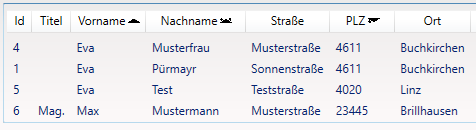
\includegraphics[scale=0.75]{images/Sortieren.png}
\end{center}
	\caption{Screenshot des Sortierens}
	\label{fig:sample}
\end{figure}
Als Grundlage zur Implementierung war ein Beispiel von Microsoft sehr hilfreich (\cite{microsoft_windows_2017}). \newline Es eine Klasse SortManager, die die Sortierung für alle Hauptseiten regelt.
\begin{lstlisting}
public SortManager SortManager { get; set; }
\end{lstlisting} 
Dazu wird im Konstruktor ein neuer SortManager initialisiert.
\begin{lstlisting}
SortManager = new SortManager();
\end{lstlisting}
Zusätzlich werden drei Events von der View abonniert. Dieses Event wird von der ListView bereitgestellt.
\begin{lstlisting}
<i:Interaction.Triggers>
	<i:EventTrigger EventName="Loaded">
		<cmd:EventToCommand Command="{Binding Initialized}"
                                        PassEventArgsToCommand="True" />
	</i:EventTrigger>
</i:Interaction.Triggers>
\end{lstlisting}
In jedem ListViewHeader werden noch Shift+LeftClick und MouseDown abonniert.
\begin{lstlisting}
<GridViewColumn DisplayMemberBinding="{Binding FirstName, UpdateSourceTrigger=PropertyChanged}">
	<GridViewColumnHeader Content="Vorname">
		<GridViewColumnHeader.InputBindings>
			<MouseBinding Gesture="Shift+LeftClick" Command="{Binding SortShift}" CommandParameter="FirstName" >
			</MouseBinding>
		</GridViewColumnHeader.InputBindings>
		<i:Interaction.Triggers>
			<i:EventTrigger EventName="MouseDown">
				<cmd:EventToCommand Command="{Binding SortCommand}"
                                        PassEventArgsToCommand="True" />
			</i:EventTrigger>
		</i:Interaction.Triggers>
	</GridViewColumnHeader>
</GridViewColumn>
\end{lstlisting}
Im ViewModel gibt es die zugehörigen ICommands:
\begin{lstlisting}
public ICommand SortCommand { get; set; }
public ICommand SortShift { get; set; }
public ICommand Initialized { get; set; }
\end{lstlisting}
Diese werden im Konstruktor initialisiert:
\begin{lstlisting}
SortCommand = new RelayCommand<RoutedEventArgs>(SortS);
SortShift = new RelayCommand<object>(SortSh);
Initialized = new RelayCommand<RoutedEventArgs>(Init);
\end{lstlisting}
Im ViewModel werden dann folgende Methoden aufgerufen:
\begin{lstlisting}
private void Init(RoutedEventArgs p)
{
	SortManager.Init(p);
}
//Click without shift key
private void SortS(RoutedEventArgs e)
{
	var tmp = this.CustomersView;
	SortManager.SortNormal(e, ref tmp);
}
//Click with shift
private void SortSh(object p)
{
	var tmp = CustomersView;
	SortManager.SortShift(p, ref tmp);
}
\end{lstlisting}
In der Methode SortManager.Init(RoutedEventArgs p) werden durch die Variable p alle GridViewColumnHeader abgespeichert. Der Grund dafür ist, dass bei dem Event SortShift keine EventArgs mitgegeben werden können, weil es sich um ein MouseBinding handelt und nicht um ein normales Event. Dadurch kann die Methode SortShift(object p, ref ICollectionView View) nicht wissen, welche Spaltenüberschrift gedrückt wurde und daher müssen am Anfang einmal alle GridViewColumnHeaders abgespeichert werden.
Wenn die Methode SortNormal(RoutedEventArgs e, ref ICollectionView View) aufgerufen wird, wird zunächst überprüft ob die Spaltenüberschrift schon einmal gedrückt wurde (dann soll nämlich die Sortierrichtung geändert werden). Wenn ja, werden die Suchrichtung sowie die Richtung des Pfeils neben der Spaltenüberschrift geändert. Ansonsten werden alle Pfeile neben den Überschriften gelöscht, die Suchrichtung auf aufsteigend gesetzt und ein neuer Pfeil gesetzt. Ein Auszug der SortNormal-Methode:
\begin{lstlisting}
//Same column pressed?
if (SortHeaders.Count == 1 && SortHeaders[0] == columnHeader)
{
	//Change sort direction
	dir = View.SortDescriptions[0].Direction;
	dir = dir == ListSortDirection.Ascending ? ListSortDirection.Descending : ListSortDirection.Ascending;
	header = ChangeArrow(columnHeader, dir, 0);
}
else
{
	//Remove arrow from old column header
	if (SortHeaders.Count > 0)
	{
		foreach (var item in SortHeaders)
		{
			item.Column.HeaderTemplate = null;
			item.Column.Width = item.ActualWidth - 20;
		}
	}
	SortHeaders.Clear();
	SortHeaders.Add(columnHeader);
	//default sort direction is ascending
	dir = ListSortDirection.Ascending;
	header = SetNewArrow(columnHeader, dir, 0);
}
View.SortDescriptions.Clear();
View.SortDescriptions.Add(new SortDescription(header, dir));
\end{lstlisting}
SortHeaders ist eine globale Variable vom Typ List\textless GridViewColumnHeader\textgreater , der die Spalten enthält, nach welchen aktuell sortiert wird. Die lokale Variable ''dir'' bezeichnet die gewünschte Sortierrichtung und ist vom Typ ListSortDirection. Der String ''header'' enthält die Property, auf die der GridViewColumnHeader bindet. Diese ist natürlich Englisch und stellt wieder ein Übersetzungsproblem dar. \newline Wie schon weiter oben erwähnt, ist der Typ ICollectionView extra für das Darstellen von Listen gemacht, deshalb enthält er auch eine Eigenschaft SortDescriptions, in welche man beliebig viele SortDescriptions einfügen kann und nach welchen die Liste automatisch sortiert wird. In den Methoden ChangeArrow und SetNewArrow wird die Spalte entsprechend breiter gemacht und das passende vorgefertigte Template gesetzt. Dieses enthält selbst designete Bilder von Pfeilen, die unter den Ressourcen des Projektes abgespeichert sind.
\begin{lstlisting}
column.Column.HeaderTemplate = Application.Current.FindResource("ArrowUp") as DataTemplate;
\end{lstlisting}
In diesem Beispiel wird dem GridViewColumnHeader column ein Pfeil der nach oben ausgerichtet ist beigefügt.
In der Methode SortShift(object p, ref ICollectionView View) wird mittels dem Parameter p der Name der Property übergeben, an die sich die Spalte bindet. Dieser wird händisch in der View übergeben (siehe oben) und ist englisch, weshalb er zuerst übersetzt werden muss. Danach wird der passende GridViewColumnHeader nach der Überschrift in den am Anfang angelegten GridViewColumnHeaders gesucht.

\begin{lstlisting}
var columnHeader = AllHeaders.Where(h => String.Equals(h.Content.ToString(), germanColumnName)).ToList().FirstOrDefault();
\end{lstlisting}
Dann wird wieder überprüft, ob dieselbe Spalte zweimal hintereinander ausgewählt wurde, sodass dann die Sortierrichtung gewechselt werden kann. Ansonsten wird überprüft ob schon drei Spalten ausgewählt wurden und wenn nicht wird eine neue Spalte zu den Sortierspalten hinzugefügt.
Auszug der SortShift-Methode:

\begin{lstlisting}
if (View.SortDescriptions.Count >= 1)
{
	ListSortDirection dir;
	int index = View.SortDescriptions.Count - 1;
	//Change sorting direction
	if (View.SortDescriptions.Count == index + 1 && View.SortDescriptions[index].PropertyName == columnName)
	{
		dir = View.SortDescriptions[index].Direction;
		dir = dir == ListSortDirection.Ascending ? ListSortDirection.Descending : ListSortDirection.Ascending;
		View.SortDescriptions.RemoveAt(index);
		View.SortDescriptions.Insert(index, new SortDescription(columnName, dir));
		ChangeArrow(columnHeader, dir, index);
		SortHeaders.Add(columnHeader);
	}
	else if (View.SortDescriptions.Count(s => s.PropertyName == columnName) == 0)
	{
	if (View.SortDescriptions.Count >= 3)
	{
		MessageBox.Show("Sie koennen maximal nach drei Spalten sortieren!", "Hinweis", MessageBoxButton.OK, MessageBoxImage.Exclamation);
		return;
	}
	dir = ListSortDirection.Ascending;
	SetNewArrow(columnHeader, dir, index+1);
	View.SortDescriptions.Add(new SortDescription(columnName, dir));
	SortHeaders.Add(columnHeader);
}
\end{lstlisting}
\section{Datenmodell}
\begin{figure}[H]
\begin{center}
	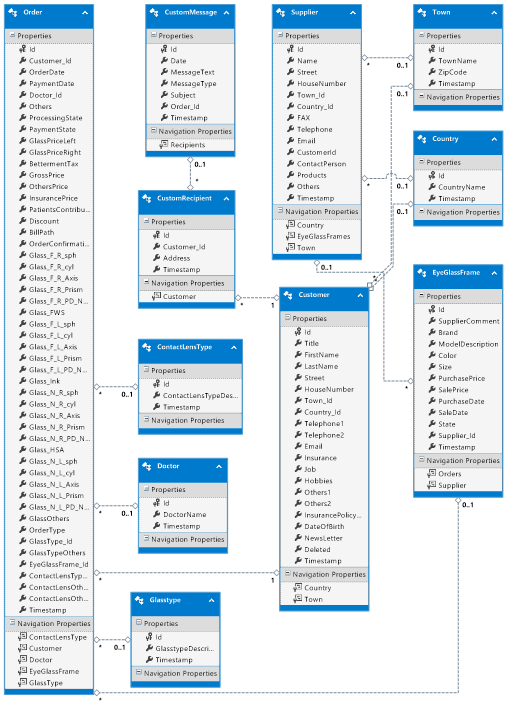
\includegraphics[scale=1.1]{images/db.png}
\end{center}
	\caption{Datenmodell}
	\label{fig:sample}
\end{figure}
Wie auch der Rest der Diplomarbeit, wurde auch das Datenmodell des Administrationsprogramms und der Website strikt getrennt. Dabei gehören die Tabellen TODO ..  der Website an und der Rest der Tabellen dem Administrationsprogramm. \newline Die Tabelle, die die meisten Felder enthält ist Tabelle der Aufträge (Order). In einem Datensatz dieser Tabelle kann entweder einen Brillenauftrag oder einen Kontaktlinsenauftrag enthalten,  was mit dem Attribut 'OrderType' gekennzeichnet ist. Falls es sich um einen Brillenauftrag handelt nimmt 'OrderType' den Wert 'B' an, ansonsten 'K'. Je nach dem um welchen Auftrag es sich handelt, kann ein Glas- bzw. Kontaktlinsentyp mit dem Auftrag verknüpft werden. In jeder der beiden Tabellen wird nur der Name des Glastyps/Kontaktlinsentyps gespeichert. Mit dem Glastyp kann beispielsweise angegeben werden, ob es sich um eine Nah- oder Fernbrille handelt. Werte in der Tabelle Kontaktlinsentyp könnten 'Weich 6 Monate' oder 'Formstabil 12 Monate' sein. \newline Falls der Auftrag ein Brillenauftrag ist, kann zusätzlich auch eine Brillenfassung vermerkt werden. In der Tabelle werden auch sämtliche Werte der Gläser gespeichert, welche die meisten Attribute in der Tabelle in Anspruch nehmen. Unter dem Attribut 'BillPath' bzw. 'OrderConfirmationPath' wird jeweils der Pfad zur letzten erstellten Rechnung/Auftragsbestätigung gespeichert. Falls der Kunde den Auftrag mit einem Augenarzt ('Doctor') in Verbindung bringen möchte, ist das ebenfalls möglich. \newline Jeder Auftrag muss einem Kunden zugewiesen werden. Die Tabelle Kunde enthält alle Grunddaten des Kunden, wobei Ort und Land in eigene Tabellen ausgelagert sind. Außerdem kann der Benutzer sonstige Informationen sowie Job oder Hobbys des Kunden speichern. Zusätzlich ist auch vermerkt, ob der Kunde Massennachrichten erhalten soll ('Newsletter') und ob der Kunde gelöscht wurde ('Deleted', siehe Kapitel 3.1.1).\newline Weiters gibt es noch die Tabellen Lieferant ('Supplier'), in der alle Informationen über einen Lieferanten gespeichert werden, wobei Ort und Land wieder in eigene Tabellen ausgelagert sind, und die Tabelle der Brillenfassungen ('EyeGlassFrame'). Diese enthält alle Informationen zu einer lagernden Brillenfassung. \newline Damit alle versendeten Nachrichten nach dem Versenden noch einmal angezeigt werden können, gibt es die Tabellen 'CustomMessage' und 'CustomRecipient'. In der Tabelle 'CustomMessage' wird das Datum sowie die Uhrzeit der Nachricht, der Text, der Typ der Nachricht (SMS oder E-Mail), der Betreff (falls es sich um eine E-Mail handelt) und die Id des Auftrages (falls es eine einzelne Nachricht ist) gespeichert. Eine solche Nachricht kann beliebig viele Empfänger haben. Die Empfänger der Nachricht müssen gesichert werden, da sonst im Nachhinein unklar ist, wer die Nachricht erhalten hat und an welche Telefonnummer bzw. E-Mail Adresse die Mitteilung versendet worden ist. Diese könnte ja seit dem Versenden der Nachricht verändert worden sein. Jeder der gespeicherten  Empfänger muss einem Kunden in der Datenbank zugeordnet sein.
\section{Projektarchitektur}
Um die Diplomarbeit so übersichtlich wie möglich zu halten, wurden fünf Projekte kombiniert.
\begin{itemize}
\item 'OpticianMgr.FillDb': Es handelt sich um eine Konsolenapplikation, welche den ConnectionString zur Datenbank enthält. Beim Start dieses Projektes wird der Inhalt der gesamten Datenbank gelöscht und mit Testdatensätzen gefüllt. Diese Daten werden zuvor in CSV-Files abgespeichert. Für jede Tabelle in der Datenbank gibt es ein CSV-File, welches eben solche selbst geschriebenen Testdatensätze beinhaltet. Ein Testdatensatz für einen Kunden könnte beispielsweise so aussehen: \newline ''Mag.;Susi;Sonne;Sonnenstraße;3;4020;Österreich;0650789456123;07242456123789; susi@gmail.com;Gebietskrankenkassa;Polizistin;Fußball;Arbeitet in Wels;Hat vormittags keine Zeit;7789031098;03.10.1998'' \newline Die einzelnen Werte der Attribute werden durch Strichpunkte getrennt. Die Reihenfolge der Werte muss für alle Datensätze dieselbe sein, deshalb wird sie meisten am Beginn des Files angeführt.
\item 'OpticianMgr.Core': Dieses Projekt enthält alle Entitäten der Datenbank, einige Interfaces sowie eine Klasse, die das Einlesen und Einfügen der Testdatensätze in die Datenbank übernimmt. \newline In dem Unterordner ''Entities'' sind die Entitäten der Datenbank sowie die Klasse ''EntityObject'' enthalten. Wie im Kapitel 2.2 schon beschrieben, erben alle Entitäten von dieser Basisklasse, sodass jede Entität eine Id und einen Timestamp besitzt. Die Klasse ''Town'' wurde beispielsweise so implementiert:
\begin{lstlisting}
namespace OpticiatnMgr.Core.Entities
{
    public class Town : EntityObject
    {
        [Required(ErrorMessage ="Bitte geben Sie einen Ortsnamen an!"), MaxLength(100, ErrorMessage ="Der Name des Ortes ist zu lange!")]
        public string TownName { get; set; }
        [Required(ErrorMessage = "Bitte geben Sie eine Postleitzahl an!"), MaxLength(15, ErrorMessage = "Die Postleitzahl ist zu lange!")]
        public string ZipCode { get; set; }
    }
}
\end{lstlisting}
Dieser Code gibt an, dass jeder Ort obligatorisch eine Bezeichnung und eine Postleitzahl haben muss. Außerdem darf die Ortsbezeichnung maximal 100 Zeichen haben und der Postleitzahl nur 15. Das ist für Fälle außerhalb von Österreich gedacht. \newline Zusätzlich beinhaltet dieses Projekt auch noch die Interfaces ''IGenericRepository'' und ''IUnitOfWork''. Deren Aufgaben wurden allerdings schon im Kapitel 2.2 beschrieben. \newline Zuletzt enthält das 'Core'-Projekt auch noch eine Klasse namens 'OpticianController'. Diese implementiert wiederum eine Methode 'FillDatabaseFromCsv()', welche die Testdatensätze der CSV-Files einlest, per LINQ konvertiert und in der Datenbank abspeichert. Um beispielsweise Testdatensätze für Orte einzulesen wird folgende Methode verwendet: 
\begin{lstlisting} 
private List<Town> GetTowns()
{
	return GetStringMatrix("TestOrte.csv").Select(o =>
	new Town()
	{
		TownName = o[1],
		ZipCode = o[0]
	}
).ToList();
}\end{lstlisting} Die Methode 'GetStringMatrix' sucht im Projektverzeichnis nach einem File mit dem übergebenen Namen und gibt ein zweidimensionales String-Array mit den Daten zurück. Mittels Linq wird jede Zeile dieses Arrays dann in einen Ort verwandelt, dessen Postleitzahl die erste Spalte des Arrays ist und die Bezeichnung die Zweite.
\item 'OpticianMgr.Persistence': Dieses Projekt beinhaltet die Klassen 'ApplicationDbContext', 'GenericRepository' und 'UnitOfWork'. Die beiden letzteren sind wesentlich Bestandteile des Data-Acces-Layers des UnitOfWork-Patterns und deshalb im Kapitel 2.2 gut beschrieben. Die Klasse 'ApplicationDbContext' beinhaltet alle DbSets der Entitäten und den ConnectionString, über welchen die Datenbank erstellt werden soll (Kapitel 2.1).
\item 'OpticianMgr.Wpf': Diese Projekt führt das Administrationsprogramm der Diplomarbeit aus. Zu den dazu notwendigen Klassen zählen in erster Linie alle Views, also alle Fenster, die der Benutzer sieht, sobald er das Programm startet. Zu jede dieser Views wurde ein ViewModel erstellt, welches den logischen Code zur View enthält. Neben den vielen ViewModels gehören dem Projekt auch alle Ressourcen und Einstellungen an, welche zur Ausführung der WPF-Applikation notwendig sind (siehe Kapitel 3.1.7 Vorgegebene Texte bearbeiten - User-Settings, 3.1.8 Filtern-'ResourceManager', 3.1.8 Sortieren - Bilder der Pfeile). \newline Weiters enthält das Projekt Klassen wie den 'VieModelLocator', welcher Referenzen zu allen ViewModels zur Verfügung stellt (Kapitel 2.5).  Außerdem gibt es noch den 'SortManager', der die Sortierung der Daten übernimmt (Kapitel 3.1.8) und den 'FileCreater', welcher zur Erstellung von Word-Dokumenten notwendig ist (Kapitel 3.1.2). \newline Um neue Fenster anzuzeigen und wieder zu schließen, wurden die Klasse 'WindowService' sowie die Interfaces 'IRequestClose' und 'IWindowService' benötigt. Der WindowService enthält für jedes Fenster, das man aus dem Programm öffnen können soll, eine Methode, welche dann wiederum die generische Methode 'ShowWindow' aufruft.
\begin{lstlisting}
public void ShowWindow<TViewModel>(TViewModel viewModel, Window newWindow) where TViewModel : IRequestClose
{
	EventHandler<EventArgs> closeHandler = null;
	closeHandler = (sender, e) =>
	{
		viewModel.CloseRequested -= closeHandler;
		newWindow.Close();
	};
	viewModel.CloseRequested += closeHandler;
	newWindow.DataContext = viewModel;
	newWindow.ShowDialog();
}
\end{lstlisting}
Wichtig ist dabei, dass das ViewModel vom Interface IRequestClose ableitet, damit das ViewModel das Event CloseRequested enthält. Diese dient dazu, dass das ViewModel, welches ein weiteres Fenster öffnet, auf das Schließen des neuen Fensters reagieren kann. 
\item 'OpticianMgr.Web': TODO
\end{itemize} 
\chapter{Selbstevaluation}\label{cha:theoretical-background}
\section{Probleme bei der Entwicklung}
\subsection{Event-Handling mit MVVM-Light}
Als Alternative zu den vielen einzelnen Fenstern für das Anlegen und Bearbeiten von Daten, wäre am Anfang eigentlich geplant gewesen, Datagrids zu benutzen. Ein Datagrid ist vergleichbar mit einer Excel-Tabelle. Das bedeutet, dass es vordefinierte Spalten gibt und die Daten in einer Tabelle darunter angezeigt werden. 
\begin{figure}[H]
\begin{center}
	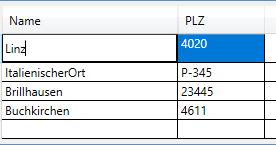
\includegraphics[scale=.75]{images/datagrid.png}
\end{center}
	\caption{Screenshot eines DataGrids}
	\label{fig:sample}
\end{figure}
\noindent Während des Entwickelns des Programmes mit DataGrids sind allerdings einige Fragen aufgekommen. Die wichtigste war: Wann werden die Daten überprüft und in die Datenbank gespeichert? Die sinnvollste Antwort auf diese Frage wäre gewesen: Nachdem der Benutzer das Feld verlässt. Allerdings wäre dazu das Abonnieren eines Events aus der View ('RowEditEnding') mittels EventToCommand von MVVM-Light notwendig gewesen, doch das war auch nach unzähligen Lösungsversuchen aus unerklärlichen Gründen nicht möglich. Grundsätzlich gibt es zwei Möglichkeiten, um Events aus der View abzufangen:
\begin{itemize}
\item Events mittels Mouse- und KeyBindings auf Commands in das ViewModel übertragen. Für Events für Maus und Tastatur ist das eine sehr praktische Lösungsmöglichkeit, allerdings können damit keine anderen Events behandelt werden.
\item Alle Events mittels MVVM-Light und der EventToCommand-Funktion ins ViewModel übertragen (Kapitel 2.5).
\end{itemize}
Das 'RowEditEnding'-Event fällt leider in die zweite Kategorie, weshalb es nicht möglich war dieses Event zu behandeln. Als Alternative wurde versucht, die Daten erst nach dem Drücken der Enter-Taste in die Datenbank zu speichern. Das wäre möglich gewesen, weil dann auf ein Event der Tastatur mittels KeyBinding reagiert werden hätte können. Doch auch diese Variante war nicht optimal, denn sobald der Benutzer einmal vergessen hätte die Enter-Taste zu betätigen, wären die Daten nicht gesichert gewesen. Aus diesem Grund wurde dann ein ganz anderer Ansatz gewählt, nämlich der der ListViews. Damit konnte das Problem des Event-Handlings umgangen werden und diese Variante ist auch benutzerfreundlicher. So öffnet sich nun zum Anlegen sowie zum Bearbeiten eines Datensatzes ein neues Fenster. \newline In der späteren Entwicklungsphase haben sich die Probleme mit MVVM-Light und EventToCommand dann aus unerfindlichen Gründen gelöst und somit konnten alle Events verwendet werden. Das war insbesondere zum Sortieren wichtig (Kapitel 3.1.8). Dennoch blieb man aber bei der Variante der neuen Fenster für das Bearbeiten und Anlegen von Daten, da es sich als viel benutzerfreundlicher erwies.
\subsection{UnitOfWork-Instanzen}
In der frühen Entwicklungsphase der Diplomarbeit traten Probleme mit dem Speichern der Daten in der Datenbank auf. Auf unerklärliche Weise wurden veränderte Daten schon vor dem eigentlichen Speichern in der UnitOfWork-Instanz geändert und somit konnten Veränderungen nie rückgängig gemacht werden. \newline Beispiel: Der Benutzer öffnet einen Kunden und möchte den Vornamen von 'Max' auf 'Maxi' ändern. Bevor er die Änderung speichert, beschließt er allerdings, dass er die Änderung doch nicht vornehmen möchte und klickt statt 'Speichern' auf 'Abbrechen'. Wenn er nun zurück auf der Startseite ist, wurde der Vorname aber trotzdem auf 'Maxi' geändert. \newline Später stellte sich heraus, dass der Grund dafür war, dass im Programm nur eine UnitOfWork-Instanz verwendet wurde und immer nur mit Referenzen von Objekten in der UnitOfWork-Instanz gearbeitet wurde. Lösungen für das Problem wären gewesen für jeden Datenbankzugriff eine neue UnitOfWork-Instanz zu erzeugen oder alle Daten, die veränderbar sein sollten, vorher lokal kopiert. Schlussendlich wurde entschieden weiterhin nur eine UnitOfWork-Instanz zu verwenden und alle veränderbaren Daten vorher lokal zu kopieren. Die andere Möglichkeit, bei der für jeden Datenbankzugriff eine neue UnitOfWork-Instanz erzeugt worden wäre, hätte den Code um einiges verlängert und unübersichtlicher gemacht. Dazu hätte für jeden Zugriff ein Using-Block verwendet werden müssen:  
\begin{lstlisting}
using(UnitOfWork uow = new UnitOfWork())
{
	Customer cus = uow.CustomerRepository.GetById(1);
}
\end{lstlisting}
% create further tex files for all other chapters of your document
\chapter{Summary}
Here you give a summary of your results and experiences. You can add also some design alternatives you considered, but kicked out later. Furthermore you might have some ideas how to drive the work you accomplished in further directions.



\bibliography{da_bibliography}{}
\bibliographystyle{alphaurl} % save alternatives are abbrvurl	alphaurl	plainurl	unsrturl

\listoffigures
\listoftables
\chapter*{Project Log Book}
\begin{tabular}{|l|l|l|l|}
\hline
Date & Participants & Todos & Due\\
\hline
\end{tabular}

\appendix
\chapter{Additional Information} \label{cha:additional-information}
\begin{comment}
If needed the appendix is the place where additional information concerning your thesis goes. Examples could be:
\begin{itemize}
	\item Source Code
	\item Test Protocols
	\item Project Proposal
	\item Project Plan
	\item Individual Goals
	\item \ldots
\end{itemize}

Again this has to be aligned with the supervisor.
\end{comment}
\chapter{Individual Goals} \label{cha:individual-goals}
This is just another example to show what content could go into the appendix.
\end{document}  